\documentclass[a4paper,13pt]{report}

\usepackage[top=2.5cm,bottom=2.5cm,left=3cm,right=2cm]{geometry}
\usepackage[a4,frame,center]{crop}
\usepackage{graphicx}
\usepackage[english]{babel}
\usepackage[utf8]{inputenc}
\usepackage[T1]{fontenc}
\usepackage{ragged2e}
\usepackage{hyphenat}
\usepackage{lmodern}
\usepackage{fancyhdr}
\usepackage[toc,page]{appendix}
\usepackage{tabularx}
\usepackage{adjustbox}
\usepackage{float}
\usepackage{amsmath}
\usepackage{indentfirst}
\usepackage[table]{xcolor}
\usepackage{array,multirow} 
\usepackage{varwidth}
\usepackage{listings}
\usepackage{background}
\usepackage{tikz}
\usepackage{hyperref}
\usepackage{ragged2e}
\usetikzlibrary{calc}
\backgroundsetup{contents={}}
\setcounter{secnumdepth}{5}

\AtBeginDocument{%
\let\mtcontentsname\contentsname
\renewcommand\contentsname{\MakeUppercase\mtcontentsname}
}

\begin{document}
    \begin{titlepage}
        \centering
        \input{border.tex}
        \LARGE{\textsc{VIETNAM AVIATION ACADEMY}}\\
        \vspace{3mm}
        \normalsize{Department of Telecommunication - Electronics Engineering Technology} \\
        \vspace{3mm}
        \large{LOCATED IN HO CHI MINH CITY} \\
        \vspace{3mm}
        
\includegraphics[scale=0.3]{img/logo.png} \\
        \vspace{3mm}
        \Large{MACHINE LEARNING AND APPLICATIONS} \\
        \vspace{10mm}
        \LARGE{\textbf{"Dangerous weapons detection using YOLOv9"}} \\ 
        \vspace{20mm}
        \normalsize{Written by} \\ 
        \vspace{3mm}
        \large{\textbf{\textit{Nguyen Van Anh Tuan}}} \\ 
        \vspace{3mm}
        \large{\textbf{\textit{Roll.No.1753020018}}} \\ 
        \vspace{15mm}
        \large{Under the guidance of} \\
        \vspace{7mm}
        \centerline{\textbf{\large{Msc.Tran Quoc Khai}}}
        \vspace{3.5cm}
        \centerline{\today}
    \end{titlepage}

    \newpage
    \thispagestyle{plain}
        \centering
        \input{border.tex}
        \LARGE{\textsc{VIETNAM AVIATION ACADEMY}}\\
        \vspace{3mm}
        \normalsize{Department of Telecommunication - Electronics Engineering Technology} \\
        \vspace{3mm}
        \large{LOCATED IN HO CHI MINH CITY} \\
        \vspace{3mm}
        
\includegraphics[scale=0.3]{img/logo.png} \\
        \vspace{3mm}
        \Large{Machine Learning and Applications} \\
        \vspace{10mm}
        \LARGE{\textbf{"DANGEGOUS WEAPONS DETECTION USING YOLOv9"}} \\ 
        \vspace{20mm}
        \normalsize{Written by} \\ 
        \vspace{3mm}
        \large{\textbf{\textit{Nguyen Van Anh Tuan}}} \\ 
        \vspace{3mm}
        \large{\textbf{\textit{Roll.No.1753020018}}} \\ 
        \vspace{15mm}
        \large{Under the guidance of} \\
        \vspace{7mm}
        \centerline{\textbf{\large{Msc.Tran Quoc Khai}}}
        \vspace{3.5cm}
        \centerline{\today}
    
    \newpage
    \thispagestyle{plain}
    \centering
    \justifying
    \centerline{\textbf{\huge{PREAMBLE}}}
    \vspace{10mm}
    \begin{flushleft}
        In today's world, terrorism remains a pervasive and evolving threat, posing significant challenges to global security and stability. The methods and tactics employed by terrorists have become increasingly sophisticated, necessitating advanced technological solutions to effectively counteract these dangers. One such critical area is the detection of dangerous weapons, which requires innovative approaches to ensure the safety of populations and the integrity of public spaces. \\ 
        \vspace{2mm}
        This report focuses on the pressing issue of contemporary terrorism and the urgent need for state-of-the-art information tools to detect and neutralize threats. Specifically, we will explore the application of \textbf{YOLOv9(You Only Look Once, version 9)}  technology in identifying dangerous weapons. \textbf{YOLOv9} represents the latest advancement in real-time object detection, offering unparalleled accuracy and speed in recognizing potential threats.
    \end{flushleft}
    \begin{flushright}
        \textbf{Auth.Nguyen Van Anh Tuan}
    \end{flushright}

    \newpage
    \thispagestyle{plain}
    \centering
    \justifying
    \centerline{\textbf{\huge{WORDS OF THANKS}}}
    \vspace{10mm}
    \begin{flushleft}
        Dear Mr.Khai, \\
        \vspace{2mm}
        I hope this message finds you well. I wanted to extend my heartfelt thanks for giving me the opportunity to write this report on contemporary terrorism and the application of YOLOv9 technology for weapon detection. Your support and trust in my capabilities have been immensely motivating. \\ 
        \vspace{2mm}
        I have tried my best to do this project. However, due to my lack of experience and 
        knowledge, there are still some unexpected mistakes in the project. Please let me know your opinions and criticizes.
        Thank you once again for this invaluable opportunity.
    \end{flushleft}
    \begin{flushright}
        \textbf{Auth.Nguyen Van Anh Tuan}
    \end{flushright}

    \newpage
    \centerline{\huge{\textbf{REVIEW OF INSTRUCTOR}}}
    \vspace{10mm}
    \noindent\makebox[\linewidth]{\rule{\paperwidth}{0.4pt}}
    \noindent\makebox[\linewidth]{\rule{\paperwidth}{0.4pt}}
    \noindent\makebox[\linewidth]{\rule{\paperwidth}{0.4pt}}
    \noindent\makebox[\linewidth]{\rule{\paperwidth}{0.4pt}}
    \noindent\makebox[\linewidth]{\rule{\paperwidth}{0.4pt}}
    \noindent\makebox[\linewidth]{\rule{\paperwidth}{0.4pt}}
    \noindent\makebox[\linewidth]{\rule{\paperwidth}{0.4pt}}
    \noindent\makebox[\linewidth]{\rule{\paperwidth}{0.4pt}}
    \noindent\makebox[\linewidth]{\rule{\paperwidth}{0.4pt}}
    \noindent\makebox[\linewidth]{\rule{\paperwidth}{0.4pt}}
    \noindent\makebox[\linewidth]{\rule{\paperwidth}{0.4pt}}
    \noindent\makebox[\linewidth]{\rule{\paperwidth}{0.4pt}}
    \noindent\makebox[\linewidth]{\rule{\paperwidth}{0.4pt}}
    \noindent\makebox[\linewidth]{\rule{\paperwidth}{0.4pt}}
    \noindent\makebox[\linewidth]{\rule{\paperwidth}{0.4pt}}
    \vspace{10mm}
    \begin{flushright}
        \today \\ 
        \vspace{5mm}
        \textbf{Instructor}
    \end{flushright}

    \newpage
    \tableofcontents
    \listoffigures

    \newpage
    \thispagestyle{plain}
    \justifying
    \centerline{\textbf{\huge{LIST OF ACRONYMS}}}
    \begin{flushleft}
        YOLO - You Only Look Once \\
        \vspace{3mm}
        OpenCV - Open source Computer Vision \\ 
        \vspace{3mm}
        PGI - Generalized Efficient Layer Aggregation Networ \\ 
        \vspace{3mm}
        GELAN - Generalized Efficient Layer Aggregation Networ \\
        \vspace{3mm}
        COCO - Common Objects in Contet \\
        \vspace{3mm}
        Val - Validation
    \end{flushleft}

    \chapter{OVERVIEW ABOUT PROJECT}

\renewcommand{\headrulewidth}{0.5pt}
\renewcommand{\footrulewidth}{0.5pt}
\thispagestyle{plain}
\pagestyle{fancy}
\fancyhf{}
\fancyhead[L]{\textbf{CHAPTER 1}}
\fancyhead[R]{\textbf{DANGEGOUS WEAPONS DETECTION USING YOLOv9}}
\raggedright
\fancyfoot[L]{From: Nguyen Van Anh Tuan}
\fancyfoot[R]{Page \thepage}

\justifying

\section{Introduction}
    In today's world, terrorism remains a pervasive and evolving threat, posing significant challenges to global security and stability. The methods and tactics employed by terrorists have become increasingly sophisticated, necessitating advanced technological solutions to effectively counteract these dangers. One such critical area is the detection of dangerous weapons, which requires innovative approaches to ensure the safety of populations and the integrity of public spaces. \\ 
    \vspace{3mm}
    This report focuses on the pressing issue of contemporary terrorism and the urgent need for state-of-the-art information tools to detect and neutralize threats. Specifically, we will explore the application of \textbf{YOLOv9(You Only Look Once, version 9)}  technology in identifying dangerous weapons. \textbf{YOLOv9} represents the latest advancement in real-time object detection, offering unparalleled accuracy and speed in recognizing potential threats.
    \vspace{3mm}
    By integrating \textbf{YOLOv9} technology into security frameworks, authorities can significantly enhance their ability to detect concealed weapons and other hazardous materials. This capability is crucial in preempting terrorist activities and mitigating the risks posed by armed attacks. Through a detailed examination of \textbf{YOLOv9} functionalities, performance metrics, and real-world applications, this report aims to underscore its potential in transforming counter-terrorism strategies.
    \vspace{3mm}
    In the following sections, we will delve into the mechanics of \textbf{YOLOv9}, its advantages over previous versions, and its practical implementation in various security scenarios. By leveraging cutting-edge technology, we can better equip our security forces to anticipate and respond to the ever-changing landscape of terrorist threats, ultimately safeguarding our societies against the scourge of terrorism.

\section{Why YOLOv9?}
    Choosing YOLOv9 over previous versions of YOLO (such as YOLOv8 or earlier) can offer several advantages. Here are some compelling reasons:
    \begin{itemize}
        \item \textbf{Improved Accuracy:} YOLOv9 typically comes with enhanced algorithms and architectures that increase the accuracy of object detection. This includes better localization of objects and more precise classification.
        \item \textbf{Higher Speed:} Despite the improved accuracy, YOLOv9 is optimized for speed, maintaining or even increasing the inference speed compared to its predecessors. This makes it suitable for real-time applications.
        \item \textbf{Advanced Features:} YOLOv9 may incorporate new features like better handling of small objects, improved multi-scale detection, and more robust handling of overlapping objects.
        \item \textbf{Better Generalization:} Enhanced training techniques and data augmentation strategies in YOLOv9 can lead to better generalization across different datasets and environments, reducing overfitting.
        \item \textbf{Reduced Computational Requirements:} YOLOv9 might offer improved efficiency, requiring less computational power or memory while achieving superior performance, making it accessible for deployment on edge devices or less powerful hardware.
        \item \textbf{Enhanced Backbone and Head Networks:} The architecture of YOLOv9 often includes more advanced backbone networks (like CSPNet, EfficientNet) and head networks that contribute to better feature extraction and object detection capabilities.
        \item \textbf{Improved Training Mechanisms:} YOLOv9 could come with advanced training methodologies such as self-supervised learning, knowledge distillation, or semi-supervised learning, improving model performance with less labeled data.
        \item \textbf{Compatibility and Integration:} YOLOv9 might offer better integration with modern frameworks, libraries, and deployment tools, facilitating easier implementation in diverse projects and workflows.
        \item \textbf{State-of-the-Art Techniques:} YOLOv9 is designed to incorporate the latest research in computer vision and deep learning, ensuring that users have access to state-of-the-art techniques and methodologies.
    \end{itemize}
    Choosing the latest version like YOLOv9 ensures that you are leveraging the most recent advancements in object detection technology, leading to improved performance and capabilities in your projects.

\section{Target and The Limits of Project}
    \subsection{Target of Project}
    This project is the first step to learn about the application of processed images in reality, at the same time is also 
    a step to deploy the learned knowledge. Through research and serious work to practice manners, as well as perfecting 
    methods, researching thinking and solving a problem. With the objectives of the project is:
    \begin{itemize}
        \item Developing an Accurate Detection Model
        \item Real-time Detection Capabilities
        \item Learn about image processing
        \item Learn about YOLO, Python
        \item Install library for YOLO, Ikomia
        \item Real-time Detection Capabilities
        \item Comprehensive Documentation and Training
        \item Write program
        \item Experimental model
        \item Developing an Accurate Detection Model
    \end{itemize}
    \subsection{Limitation of Project}
    \begin{itemize}
        \item The limitation of this project is the inability to detect weapons when processing through colorless video
        \item Cannot detect when the distance of the object is too far from the camera
        \item There is no device powerful enough to be able to train on a huge amount of data
        \item Limitation of Google Colab environment when using too much GPU
    \end{itemize}

\section{Workflow of Project}
    \begin{figure}[H]
        \centering
        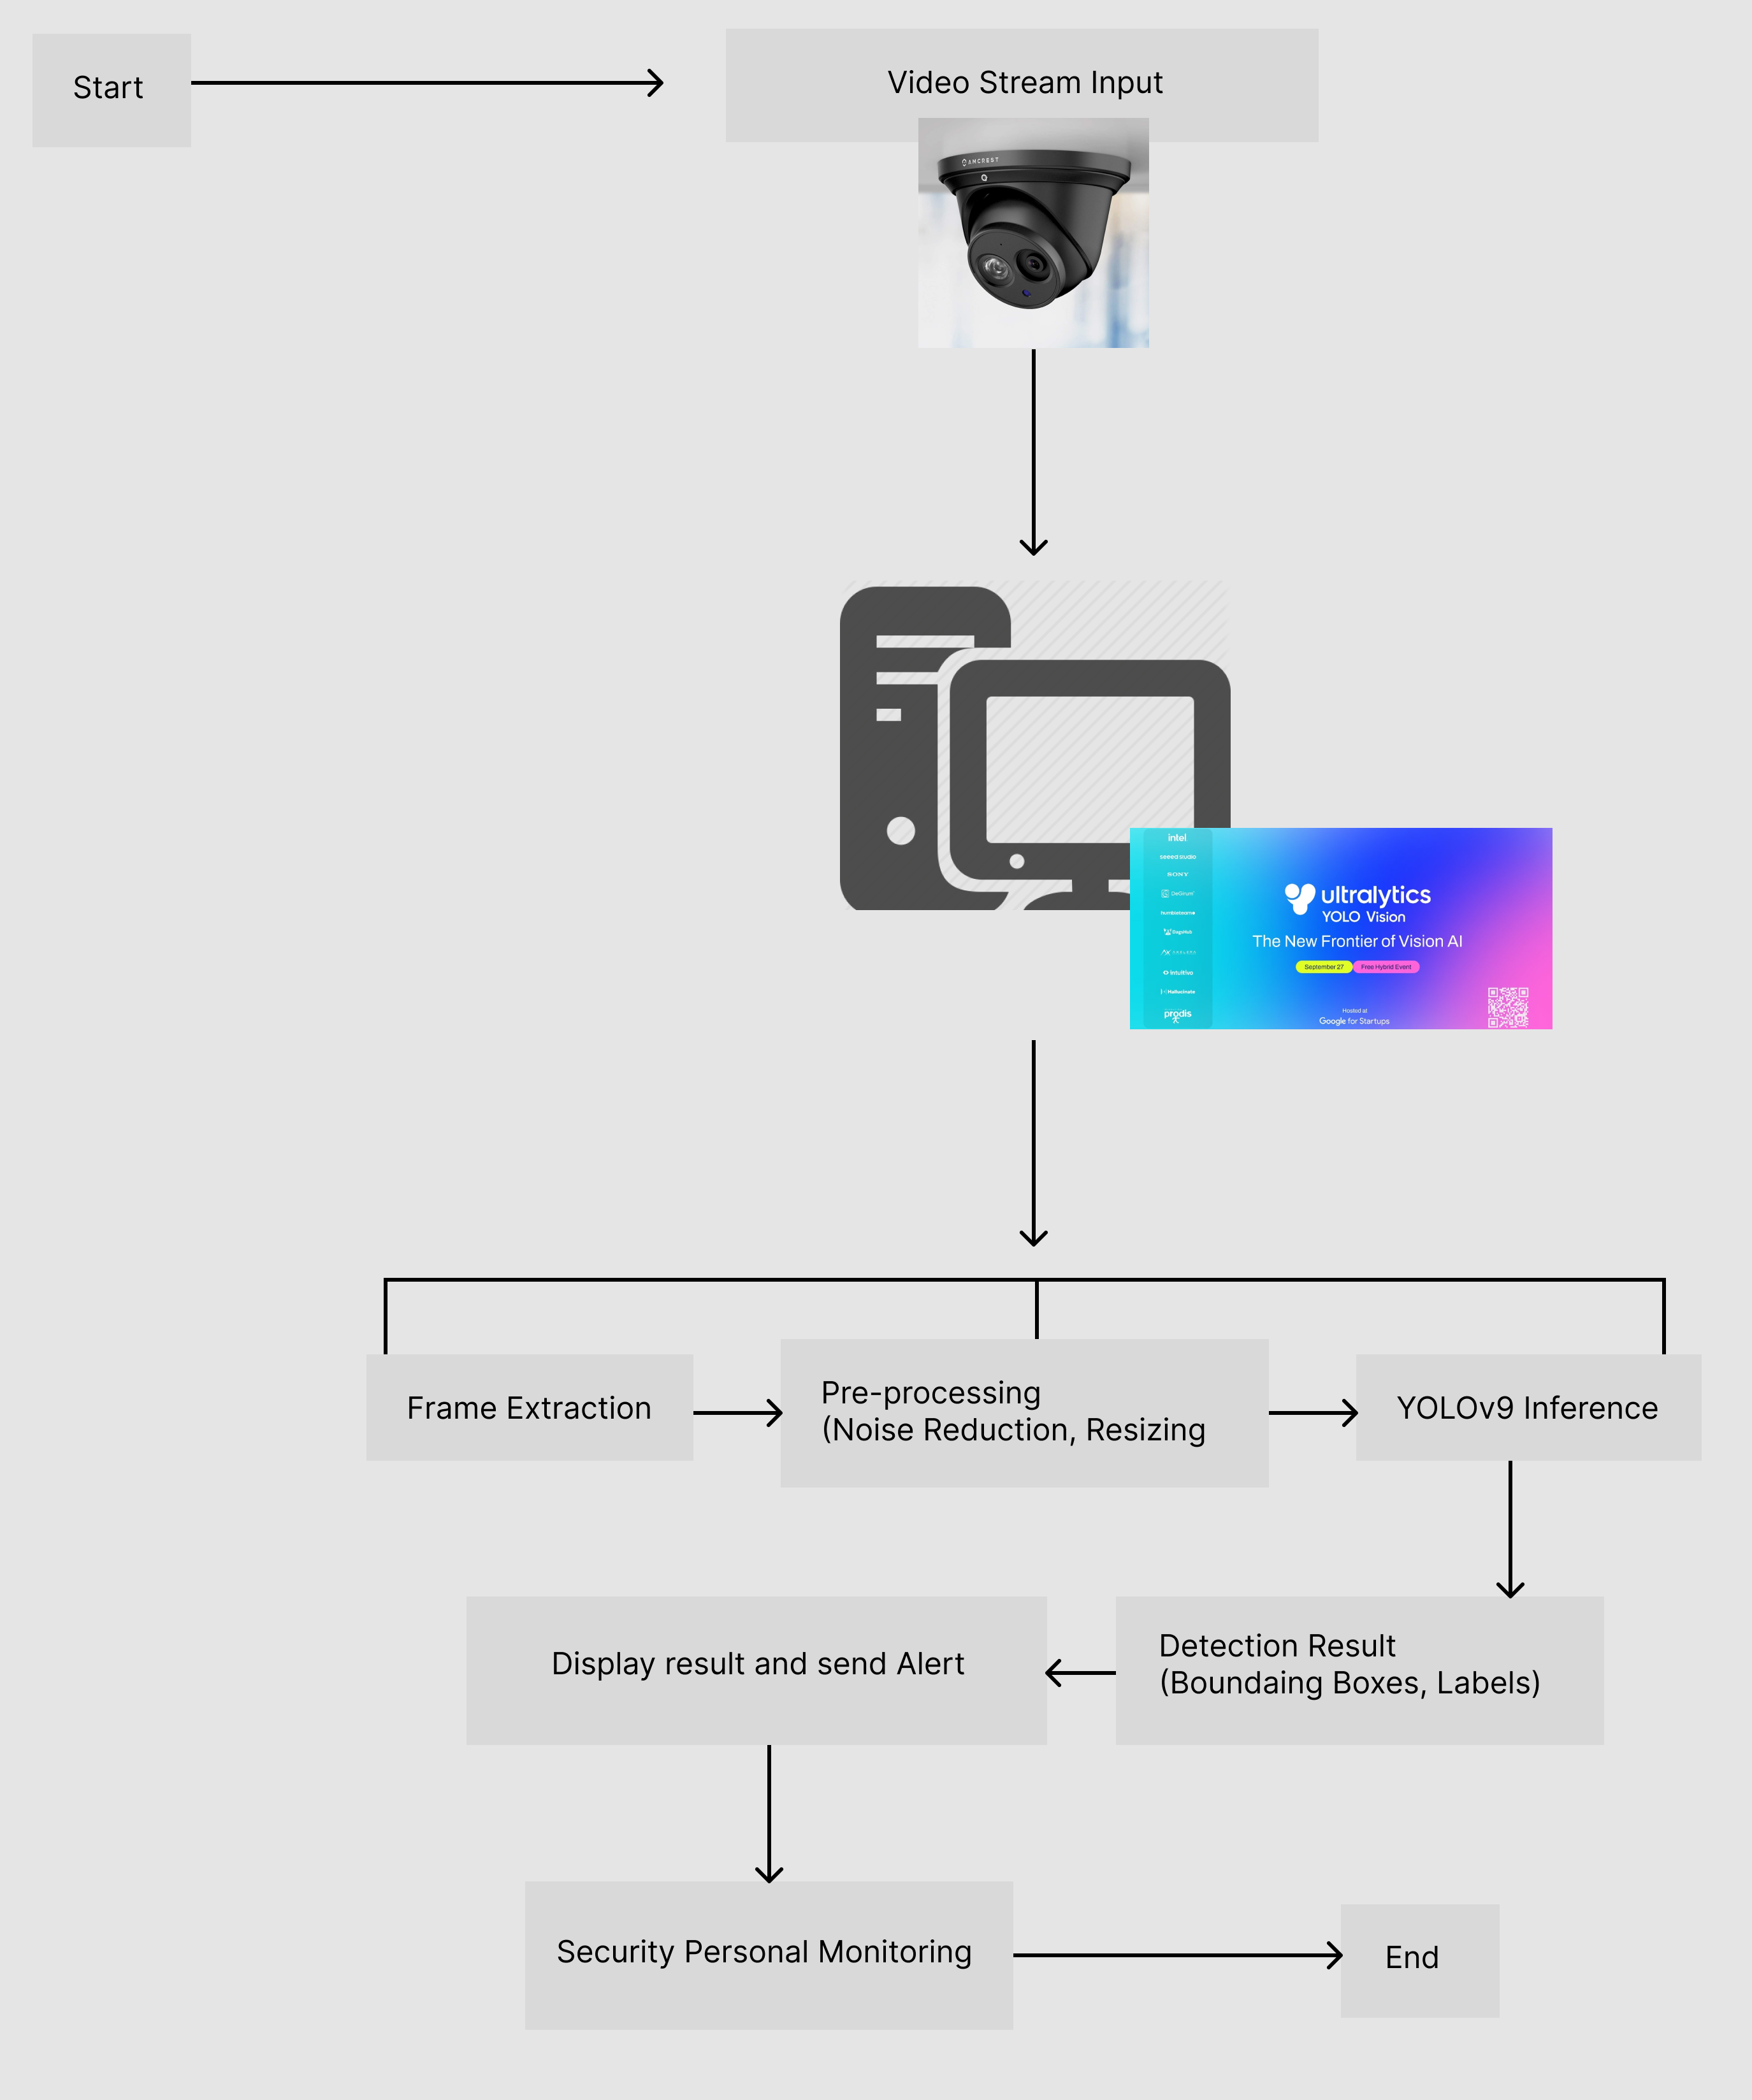
\includegraphics[width=0.8\linewidth]{img/Diagram.png}
        \caption{Block Diagram of Project}
        \label{fig:diagram}
    \end{figure}

    \chapter{THEORETICAL BASIS}

\renewcommand{\headrulewidth}{0.5pt}
\renewcommand{\footrulewidth}{0.5pt}
\thispagestyle{plain}
\pagestyle{fancy}
\fancyhf{}
\fancyhead[L]{\textbf{CHAPTER 2}}
\fancyhead[R]{\textbf{DANGEGOUS WEAPONS DETECTION USING YOLOv9}}
\raggedright
\fancyfoot[L]{From: Nguyen Van Anh Tuan}
\fancyfoot[R]{Page \thepage}

\justifying

\section{Overview about YOLOv9}
    \begin{figure}[H]
        \centering
        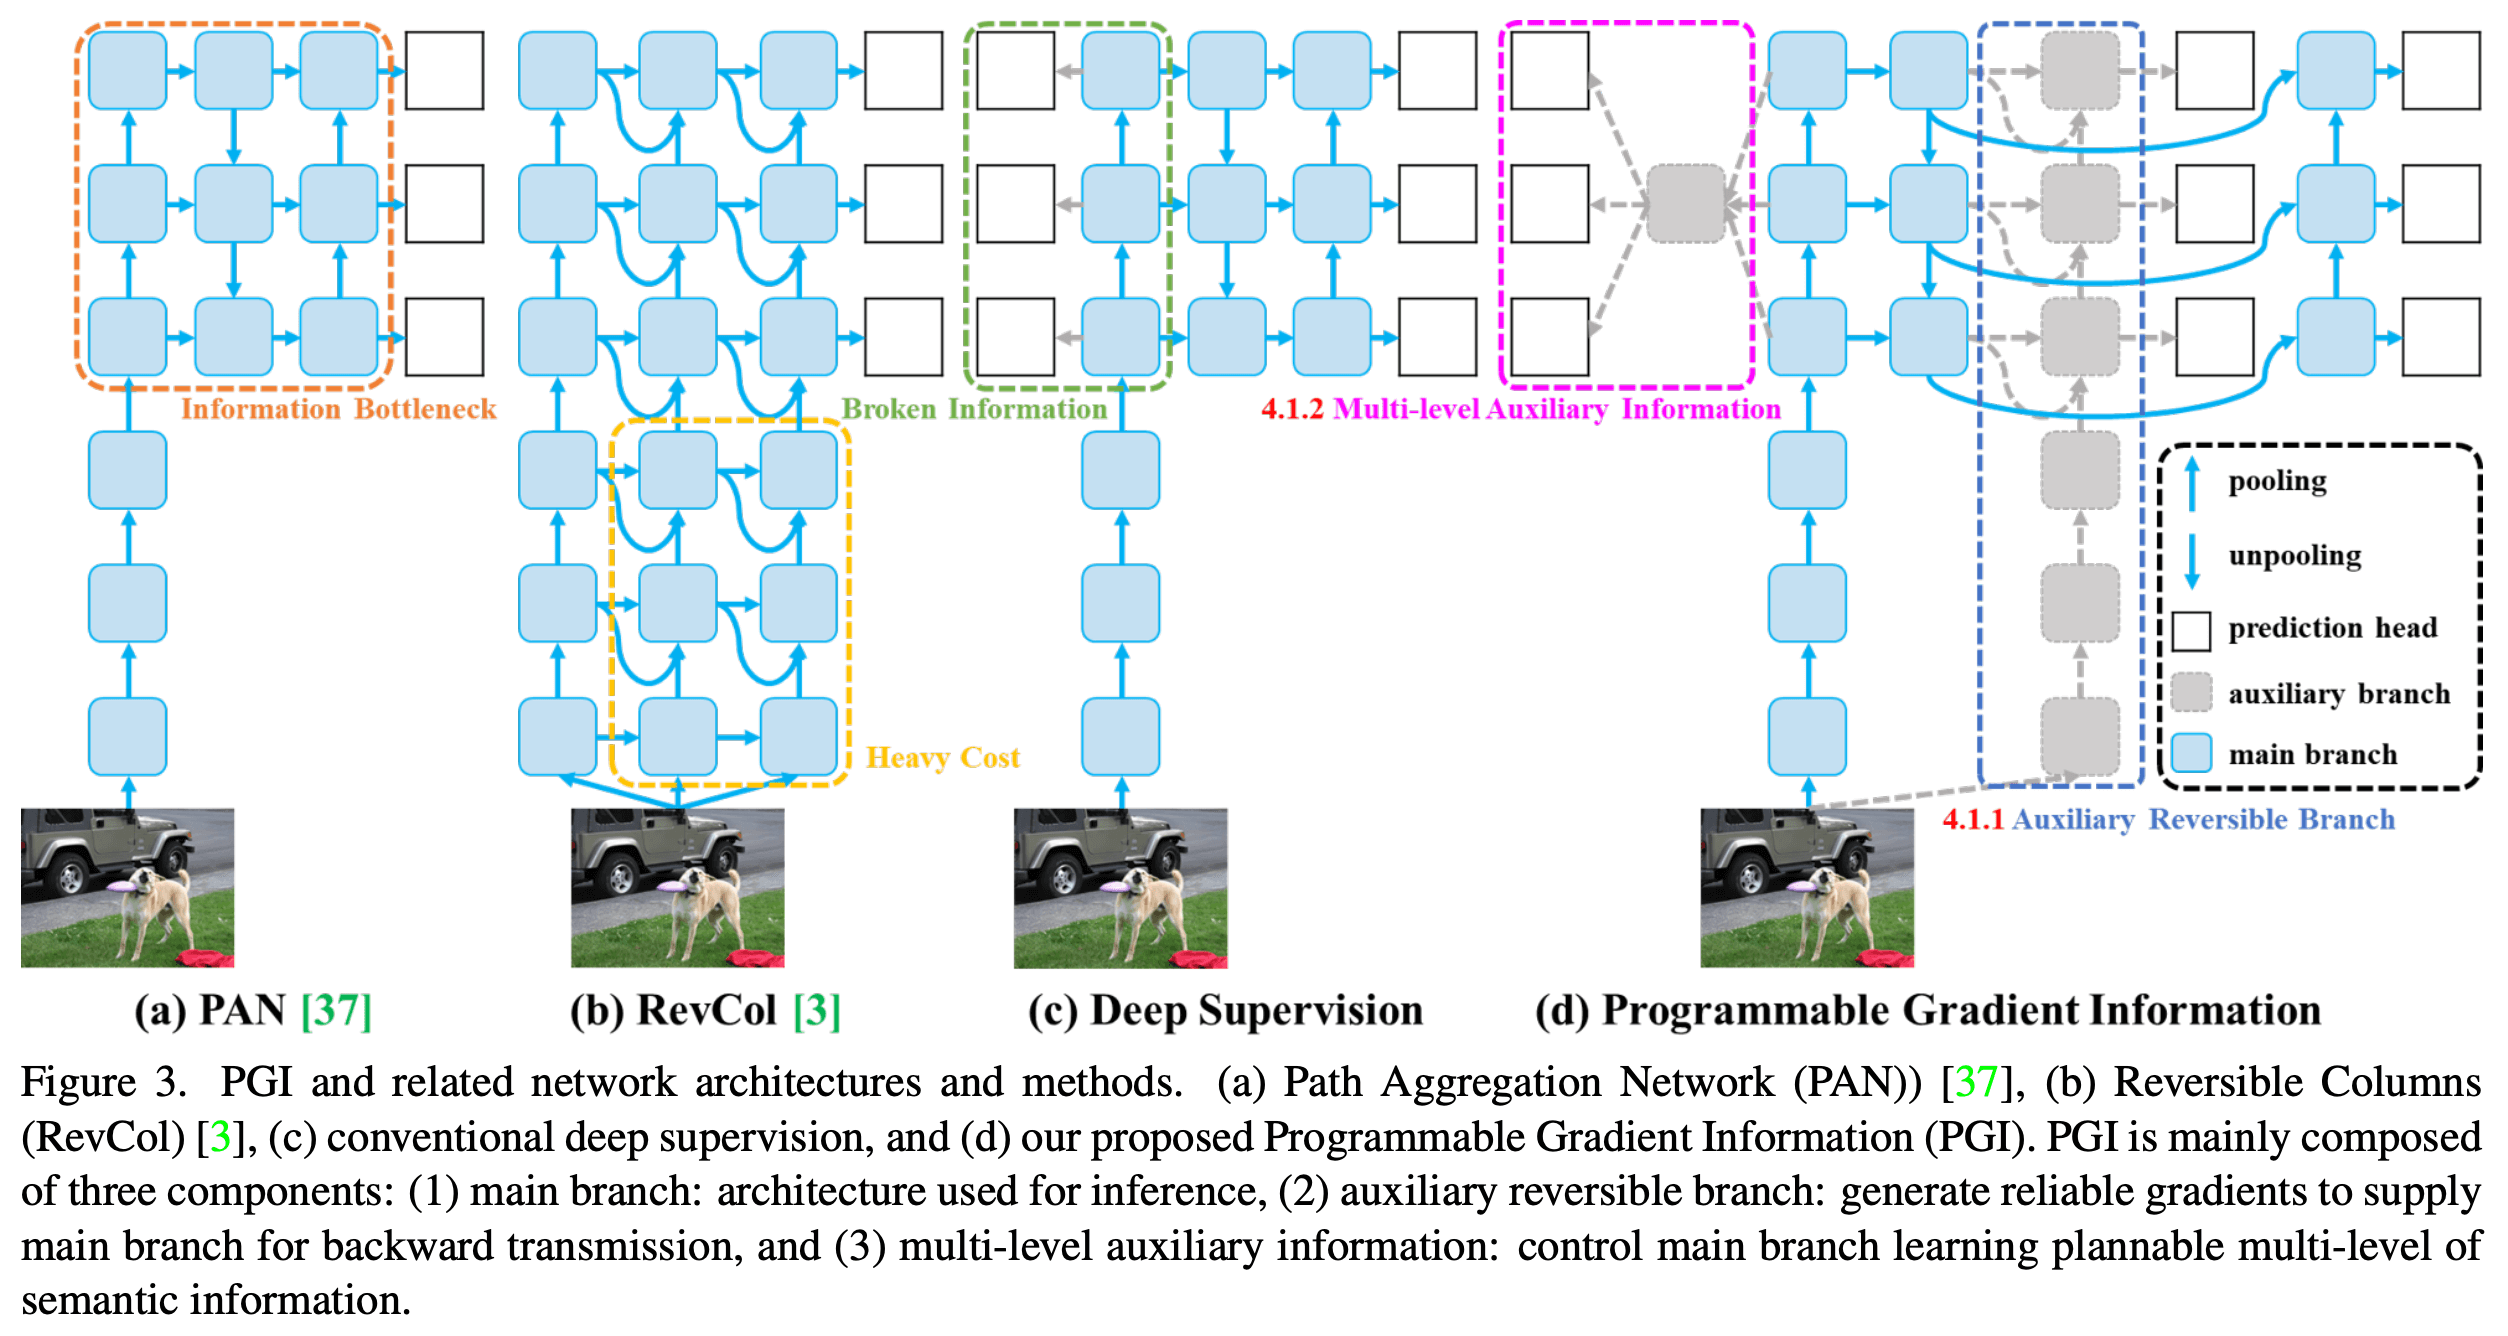
\includegraphics[width=0.8\linewidth]{img/core_innovation.png}
        \caption{PGI and related network architectures and methods. }\
        \label{fig:PGI}
    \end{figure}
    With the continuous evolution of computer vision technologies, YOLOv9 emerges as the latest advancement, developed by Chien-Yao
    Wang, I-Hau Yeh, and Hong-Yuan Mark Liao. This trio of researchers has a rich history in the field, having contributed to the
    development of preceding models such as YOLOv4, YOLOR, and YOLOv7. \\
    \begin{figure}[H]
        \centering
        
\includegraphics[width=0.8\linewidth]{img/ultralytics.jpg}
        \caption{Ultralytics's logo}
    \end{figure}
    YOLOv9 marks a significant advancement in real-time object detection, introducing groundbreaking techniques such as Programmable
    Gradient Information (PGI) and the Generalized Efficient Layer Aggregation Network (GELAN). This model demonstrates remarkable
    improvements in efficiency, accuracy, and adaptability, setting new benchmarks on the MS COCO dataset. \\
    \begin{figure}[H]
        \centering
        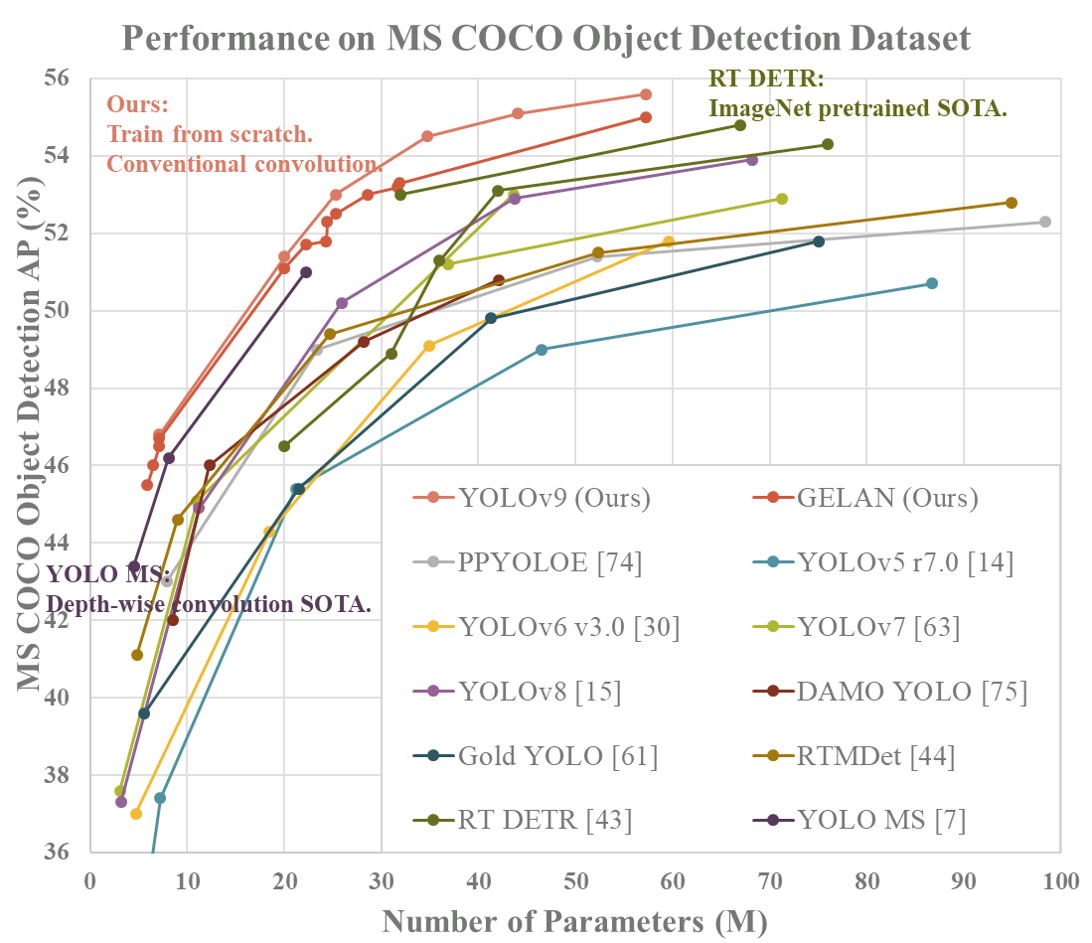
\includegraphics[width=0.8\linewidth]{img/performance_yolov9.png}
        \caption{Comparisons of the real-time object detecors on MS COCO dataset}
    \end{figure}
    In the quest for optimal real-time object detection, YOLOv9 stands out with its innovative approach to overcoming information loss
    challenges inherent in deep neural networks. By integrating PGI and the versatile GELAN architecture, YOLOv9 not only enhances the
    model's learning capacity but also ensures the retention of crucial information throughout the detection process, thereby achieving
    exceptional accuracy and performance.

\section{Methodology}
    \subsection{Programmable Gradient Information (PGI)}
        In order to solve the aforementioned problems, it was proposed 
        a new auxiliary supervision framework called Programmable 
        Gradient Information (PGI), as shown in Figure \ref{fig:PGI}.
        PGI mainly includes three components, namely
        (1) main branch, (2) auxiliary reversible branch, and (3)
        multi-level auxiliary information. From Figure \ref{fig:PGI} we
        see that the inference process of PGI only uses main branch
        and therefore does not require any additional inference cost.
        As for the other two components, they are used to solve or
        slow down several important issues in deep learning methods. 
        Among them, auxiliary reversible branch is designed
        to deal with the problems caused by the deepening of neural
        networks. Network deepening will cause information bottleneck, 
        which will make the loss function unable to generate reliable
        gradients. As for multi-level auxiliary information, it is designed
        to handle the error accumulation problem
        caused by deep supervision, especially for the architecture
        and lightweight model of multiple prediction branch. Next,
        we will introduce these two components step by step
        \subsubsection{Auxiliary Reversible Branch}
            In PGI, it was proposed auxiliary reversible branch to generate 
            reliable gradients and update network parameters. By
            providing information that maps from data to targets, the
            loss function can provide guidance and avoid the possibility 
            of finding false correlations from incomplete feed forward 
            features that are less relevant to the target. We propose
             the maintenance of complete information by introducing
             reversible architecture, but adding main branch to reversible
             architecture will consume a lot of inference costs.
            We analyzed the architecture of \ref{fig:PGI} and found that
            when additional connections from deep to shallow layers
            are added, the inference time will increase by 20\%. When
            we repeatedly add the input data to the high-resolution computing
            layer of the network (yellow box), the inference time
            even exceeds twice the time.
            \begin{figure}[H]
                \centering
                \includegraphics[width=0.8\linewidth]{img/GELAN.png}
                \caption{The architecture of GELAN: (a) CSPNet [64], (b) ELAN [65], and (c) proposed GELAN. We imitate CSPNet and extend ELAN into GELAN that can support any computational blocks}
                \label{fig:GELAN}
            \end{figure}
            Finally, since auxiliary reversible branch can be removed
            during the inference phase, the inference capabilities of the
            original network can be retained. We can also choose any
            reversible architectures in PGI to play the role of auxiliary
            reversible branch
        \subsubsection{Multi-level Auxiliary Information}
            In this section we will discuss how multi-level auxiliary in-
            formation works. The deep supervision architecture includ-
            ing multiple prediction branch is shown in \ref{fig:PGI}. For
            object detection, different feature pyramids can be used to
            perform different tasks, for example together they can de-
            tect objects of different sizes. Therefore, after connecting
            to the deep supervision branch, the shallow features will be
            guided to learn the features required for small object detec-
            tion, and at this time the system will regard the positions
            of objects of other sizes as the background. However, the
            above deed will cause the deep feature pyramids to lose a lot
            of information needed to predict the target object. Regard-
            ing this issue, we believe that each feature pyramid needs
            to receive information about all target objects so that subse-
            quent main branch can retain complete information to learn
            predictions for various targets.\\
            \vspace{3mm}
            The concept of multi-level auxiliary information is to in-sert
            an integration network between the feature pyramid hi-
            erarchy layers of auxiliary supervision and the main branch,
            and then uses it to combine returned gradients from differ-
            ent prediction heads, as shown in Figure 3 (d). Multi-level
            auxiliary information is then to aggregate the gradient infor-
            mation containing all target objects, and pass it to the main
            branch and then update parameters. At this time, the charac-
            teristics of the main branch’s feature pyramid hierarchy will
            not be dominated by some specific object’s information. As
            a result, our method can alleviate the broken information
            problem in deep supervision. In addition, any integrated
            network can be used in multi-level auxiliary information.
            Therefore, plan the required semantic levels to guide
            the learning of network architectures of different sizes.
    \subsection{Generalized Efficient Layer Aggregation Network (GELAN)}
        \subsubsection{Generalized ELAN}
            For GELAN, first do ablation studies for computational
            blocks. Used Res blocks [21], Dark blocks [49], and
            CSP blocks [64] to conduct experiments, respectively. \ref{tab:GELAN}
            shows that after replacing convolutional layers in
            ELAN with different computational blocks, the system can
            maintain good performance. Users are indeed free to re-
            place computational blocks and use them on their respective
            inference devices. Among different computational block re-
            placements, CSP blocks perform particularly well. They
            not only reduce the amount of parameters and computation,
            but also improve AP by 0.7\%. Therefore, choose CSP-
            ELAN as the component unit of GELAN in YOLOv9. \\
            \begin{table}[ht]
                \centering
                \begin{tabular}{| l | l | l | l | l |}
                    \hline
                    \rowcolor{lightgray} Model & CB type & \#Param. & FLOPs & AP${^{val}_{50:95}}$ \\ \hline
                    GELAN-S & Conv & 6.2M & 23.5G & 44.8\% \\ \hline
                    GELAN-S & Res [21] & 5.4M & 21.0G & 44.3\% \\ \hline
                    GELAN-S & Dark [49] & 5.7M & 21.8G & 44.5\% \\ \hline
                    GELAN-S & CSP [64] & 5.9M & 22.4G & 45.5\% \\ \hline
                \end{tabular}
                \caption{Ablation study on various computational blocks}
                \label{tab:GELAN}
            \end{table}
            Next, conduct ELAN block-depth and CSP block-
            depth experiments on GELAN of different sizes, and display
            the results in \ref{tab:ELAN-CSP}. We can see that when the depth
            of ELAN is increased from 1 to 2, the accuracy is significantly
            improved. But when the depth is greater than or
            equal to 2, no matter it is improving the ELAN depth or the
            CSP depth, the number of parameters, the amount of computation,
            and the accuracy will always show a linear relationship.
            This means GELAN is not sensitive to the depth.
            In other words, users can arbitrarily combine the components
            in GELAN to design the network architecture, and
            have a model with stable performance without special design.
            In \ref{tab:ELAN-CSP}, for YOLOv9-{S,M,C}, set the pairing
            of the ELAN depth and the CSP depth to {{2, 3}, {2, 1},
            {2, 1}}. \\
            \vspace{3mm}
            GELAN represents a strategic architectural advancement, enabling YOLOv9 to achieve superior parameter utilization and computational efficiency. Its design allows for flexible integration of various computational blocks, making YOLOv9 adaptable to a wide range of applications without sacrificing speed or accuracy.
            \begin{table}[ht]
                \centering
                \begin{tabular}{| l | l | l | l | l | l |}
                    \hline
                    \rowcolor{lightgray} Model & $D_{ELAN}$ & $D_{CSP}$ & \#Param. & FLOPs & AP${^{val}_{50:95}}$ \\ \hline
                    GELAN-S & 2 & 1 & 5.9M & 22.4G & 45.5\% \\ 
                    GELAN-S & 2 & 2 & 6.5M & 24.4G & 46.0\% \\ 
                    GELAN-S & 3 & 1 & 7.1M & 26.3G & 46.5\% \\ 
                    GELAN-S & 2 & 3 & 7.1M & 26.4G & 46.7\% \\ \hline
                    GELAN-M & 2 & 1 & 20.0M & 76.3G & 51.1\% \\ 
                    GELAN-M & 2 & 2 & 22.2M & 85.1G & 51.7\% \\ 
                    GELAN-M & 3 & 1 & 24.3M & 93.5G & 51.8\% \\ 
                    GELAN-M & 2 & 3 & 24.4M & 94.0G & 52.3\% \\ \hline
                    GELAN-C & 1 & 1 & 18.9M & 76.3G & 51.1\% \\ 
                    GELAN-C & 2 & 1 & 25.3M & 85.1G & 51.7\% \\ 
                    GELAN-C & 2 & 2 & 28.6M & 93.5G & 51.8\% \\
                    GELAN-C & 3 & 1 & 31.7M & 93.5G & 51.8\% \\
                    GELAN-C & 2 & 3 & 31.9M & 94.0G & 52.3\% \\ \hline
                \end{tabular}
                \caption{Ablation study on ELAN and CSP depth}
                \label{tab:ELAN-CSP}
            \end{table}
            \begin{figure}[H]
                \centering
                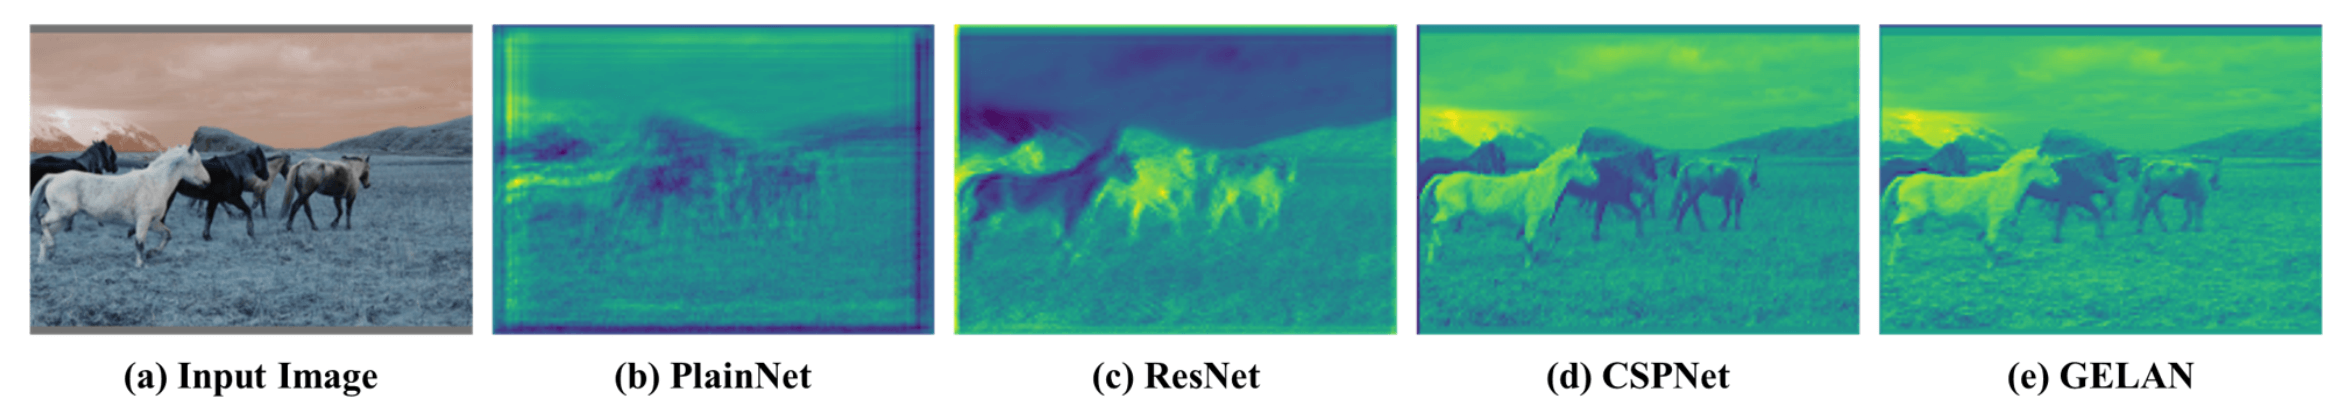
\includegraphics[width=0.8\linewidth]{img/gelan.png}
                \caption{Visualization results of random initial weight output feature maps for different network architectures: (a) input image, (b)PlainNet, (c) ResNet, (d) CSPNet, and (e) proposed GELAN. From the figure, we can see that in different architectures, the information provided to the objective function to calculate the loss is lost to varying degrees, and our architecture can retain the most complete information and provide the most reliable gradient information for calculating the objective function.}
                \label{fig:gelan}
            \end{figure}
    \subsection{Implimentation Details}
        \begin{figure}[H]
            \centering
            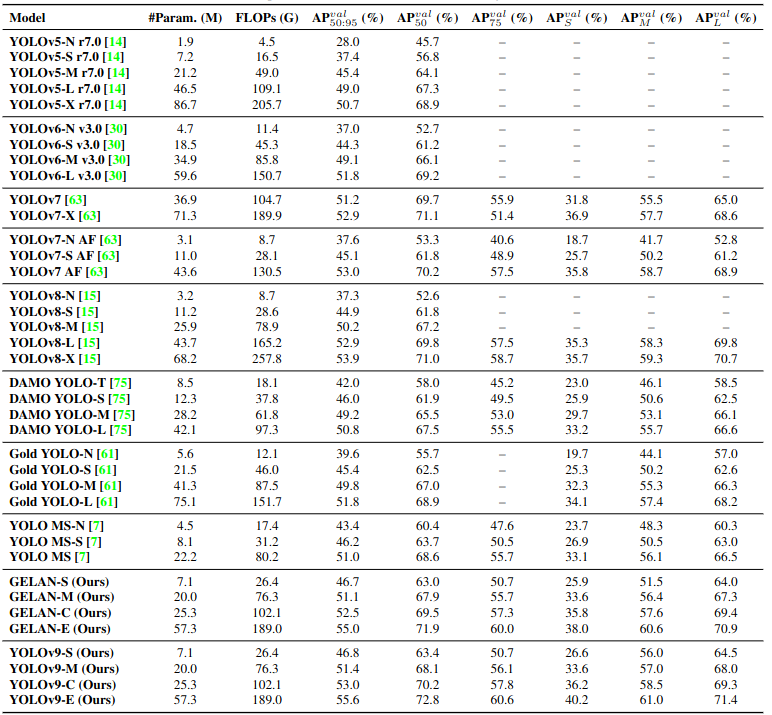
\includegraphics[width=0.9\linewidth]{img/comparison.png}
            \caption{Comparison of state-of-the-art real-time object detectors}
            \label{fig:comparison}
        \end{figure}
        \begin{figure}[H]
            \centering
            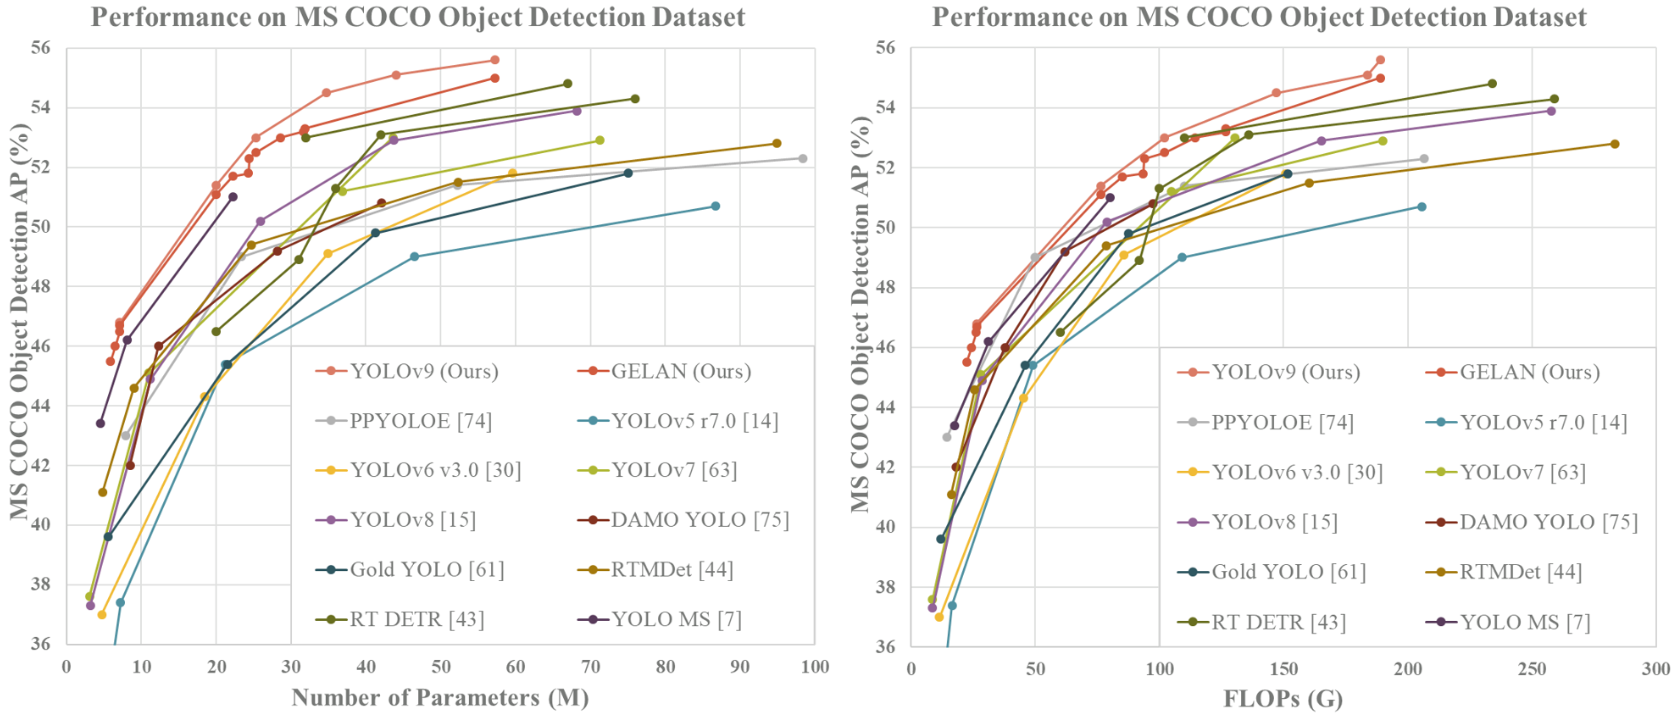
\includegraphics[width=0.9\linewidth]{img/tate-of-the-art_real-time.png}
            \caption{Comparison of state-of-the-art real-time object detectors. The methods participating in the comparison all use ImageNet as pre-trained weights, including RT DETR [43], RTMDet [44], and PP-YOLOE [74], etc. The YOLOv9 that uses train-from-scratch method clearly surpasses the performance of other methods.}
            \label{fig:state-of-the-art}
        \end{figure}

\section{Python Programming Language}
    \subsection{Introduce About Python Programming Language}
        \begin{figure}[H]
            \centering
            
\includegraphics[width=0.8\linewidth]{img/python-logo.jpg}
            \caption{Python Programming Language}
            \label{fig:python}
        \end{figure}
        Python is an interpreted high-level general-purpose programming language. Python's design philosophy emphasizes code readability 
        with its notable use of significant indentation. Its language constructs as well as its object-oriented approach aim to help programmers 
        write clear, logical code for small and large-scale projects. \\
        \vspace{3mm}
        Python is dynamically-typed and garbage-collected. It supports multiple programming paradigms, including structured (particularly, procedural), 
        object-oriented and functional programming. Python is often described as a "batteries included" language due to its comprehensive standard library. \\
        \vspace{3mm}
        Python is completely dynamically typed and uses automatic memory allocation, so it's similar to Perl, Ruby, Scheme, SmallTalk, and TCL. Python is 
        developed in an open-source project, managed by the non-profit Python Software Foundation. \\
        \vspace{3mm}
        Originally, Python was developed to run on the Unix platform. But then over time, Python gradually expanded to all operating systems from MS DOS to 
        Mac OS, OS/2, Windows, Linux and other operating systems of the Unix family.
    \subsection{Applications}
        Python is used in many different fields: 
        \begin{enumerate}
            \item Web Development: Python provide many framworks to choose for development, Django framwork. Udacity, Youtube, Dropbox is built (in large part) by using Python.
            \item Game Development: Pygame, but Python is not a best choice to to developed game.
            \item Machine Learning: Theano, Tensorflow, Scikit-learn... 
            \item Computer Science: OpenCV, Numpy, Pandas, Scipy... 
            \item IoT: Arduino, Raspberry Pi 
        \end{enumerate}

\section{Ikomia}
    \subsection{About The Project}
        Ikomia API is an open source dev tool designed to simplify the development and deployment of Computer Vision solutions. It enables effortless integration of state-of-the-art algorithms from multiple sources, such as \textbf{OpenCV, Detectron2, OpenMMLab}, and \textbf{YOLO}, into your projects. \\
        \vspace{3mm}
        With Ikomia API, you can focus on building powerful and innovative Computer Vision applications without worrying about the complexities of managing dependencies and integrating different frameworks. The API handles the download, installation and management of the selected algorithms, enabling the creation of customized solutions with minimal coding effort. \\
        \vspace{3mm}
        Whether you’re a seasoned developer or new to the field of Computer Vision, Ikomia API provides an accessible and efficient way to stay up-to-date with the latest advancements and bring your ideas to life.
    \subsection{Key Features}
        \begin{itemize}
            \item \textbf{Ease of use:} Quickly integrate state-of-the-art Computer Vision algorithms into your projects with just a few lines of code.
            \item \textbf{Cross-platform:} Compatible with Windows and Linux operating systems.
            \item \textbf{Support for popular frameworks:} Seamlessly use popular frameworks like OpenCV, Detectron2, OpenMMLab, and YOLO.
            \item \textbf{Automatic dependency management:} Ikomia API automatically downloads, installs, and manages the requirements for the chosen algorithms.
            \item \textbf{Modular design:} Easily mix and match algorithms from different repositories to create custom solutions.
            \item \textbf{Open source:} Benefit from the collaborative development and transparency of an open source project.
            \item \textbf{Regular updates:} Stay up-to-date with the latest Computer Vision advancements through frequent releases and updates.
        \end{itemize}

    \chapter{RELATED WORKS}

\renewcommand{\headrulewidth}{0.5pt}
\renewcommand{\footrulewidth}{0.5pt}
\thispagestyle{plain}
\pagestyle{fancy}
\fancyhf{}
\fancyhead[L]{\textbf{CHAPTER 3}}
\fancyhead[R]{\textbf{DANGEGOUS WEAPONS DETECTION USING YOLOv9}}
\raggedright
\fancyfoot[L]{From: Nguyen Van Anh Tuan}
\fancyfoot[R]{Page \thepage}

\justifying

\section{Collect Dataset}
    \subsection{Choose Type of Dataset}
        Nowaday, on market, there are many type of dataset format we can use for training model purpose. For detection, we will have a lot of dataset format like:
        \begin{itemize}
            \item Argoverse
            \item COCO
            \item LVIS
            \item COCO8
            \item GlobalWheat2020
            \item Objects365
            \item OpenImagesV7
            \item SKU-110K
            \item VOC
            \item xView
            \item Roboflow 100
            \item Brain-tumor
            \item African-wildlife 
            \item Signature
        \end{itemize}
        For segmentation, we will have:
        \begin{itemize}
            \item COCO 
            \item COCO8-seg 
            \item Crack-seg 
            \item Carparts-seg 
            \item Package-seg 
        \end{itemize}
        For pose, we will have:
        \begin{itemize}
            \item COCO
            \item COCO8-pose
            \item Tiger-pose
        \end{itemize}
        For classification, we have:
        \begin{itemize}
            \item Caltech 101 
            \item Caltech 256
        \end{itemize}
        In this project, i'll choose COCO dataset work with it.
        \subsubsection{Overview COCO Dataset}
            The \textbf{COCO (Common Objects in Context)} dataset is a large-scale object detection, segmentation, and captioning dataset. It is designed to encourage research on a wide variety of object categories and is commonly used for benchmarking computer vision models. It is an essential dataset for researchers and developers working on object detection, segmentation, and pose estimation tasks.
            \begin{figure}[H]
                \centering
                
\includegraphics[width=0.8\linewidth]{img/coco-logo.png}
                \caption{COCO Dataset}
                \label{fig:coco}
            \end{figure}
        \subsubsection{COCO Pretrained Models}
            \begin{table}[ht]
                \centering
                \begin{adjustbox}{width=\textwidth}
                \small
                \begin{tabular}{| c | c | c | c | c | c | c |}
                    \hline
                    \rowcolor{lightgray} Model & Size (pixels) & mAP${^{val}_{50:95}}$ & Speed CPU ONNX (ms) & Speed A100 TensorRT (ms) & params (M) & FLOPs (B) \\ \hline
                    YOLOv8n & 640 & 37.3 & 80.4 & 0.99 & 3.2 & 8.7 \\ \hline
                    YOLOv8s & 640 & 44.9 & 128.4 & 1.20 & 11.2 & 28.6 \\ \hline
                    YOLOv8m & 640 & 50.2 & 234.7 & 1.83 & 25.9 & 78.9 \\ \hline
                    YOLOv8l & 640 & 52.9 & 375.2 & 2.39 & 43.7 & 165.2 \\ \hline
                    YOLOv8x & 640 & 53.9 & 479.1 & 3.53 & 68.2 & 257.8 \\ \hline
                \end{tabular}
                \end{adjustbox}
                \caption{COCO Pretrained Models}
                \label{tab:coco-pretrained}
            \end{table}
        \subsubsection{Key Feature}
            COCO is a large-scale object detection, segmentation, and captioning dataset. COCO has several features:
            \begin{itemize}
                \item Object segmentation
                \item Recognition in context
                \item Superpixel stuff segmentation
                \item 330K images (>200K labeled)
                \item 1.5 million object instances
                \item 80 object categories
                \item 91 stuff categories
                \item 5 captions per image
                \item 250,000 people with keypoints
            \end{itemize}
        \subsubsection{Data Structure}
            The COCO dataset is split into three subsets:
            \begin{enumerate}
                \item \textbf{Train2017:} This subset contains 118K images for training object detection, segmentation, and captioning models.
                \item \textbf{Val2017:} This subset has 5K images used for validation purposes during model training.
                \item \textbf{Test2017:} This subset consists of 20K images used for testing and benchmarking the trained models. Ground truth annotations for this subset are not publicly available, and the results are submitted to the COCO evaluation server for performance evaluation.
            \end{enumerate}
        \subsubsection{Applications}
            The COCO dataset is widely used for training and evaluating deep learning models in object detection (such as YOLO, Faster R-CNN, and SSD), instance segmentation (such as Mask R-CNN), and keypoint detection (such as OpenPose). The dataset's diverse set of object categories, large number of annotated images, and standardized evaluation metrics make it an essential resource for computer vision researchers and practitioners.
        \subsubsection{Sample Images and Annotations}
            The COCO dataset contains a diverse set of images with various object categories and complex scenes. Here are some examples of images from the dataset, along with their corresponding annotations:
            \begin{figure}[H]
                \centering
                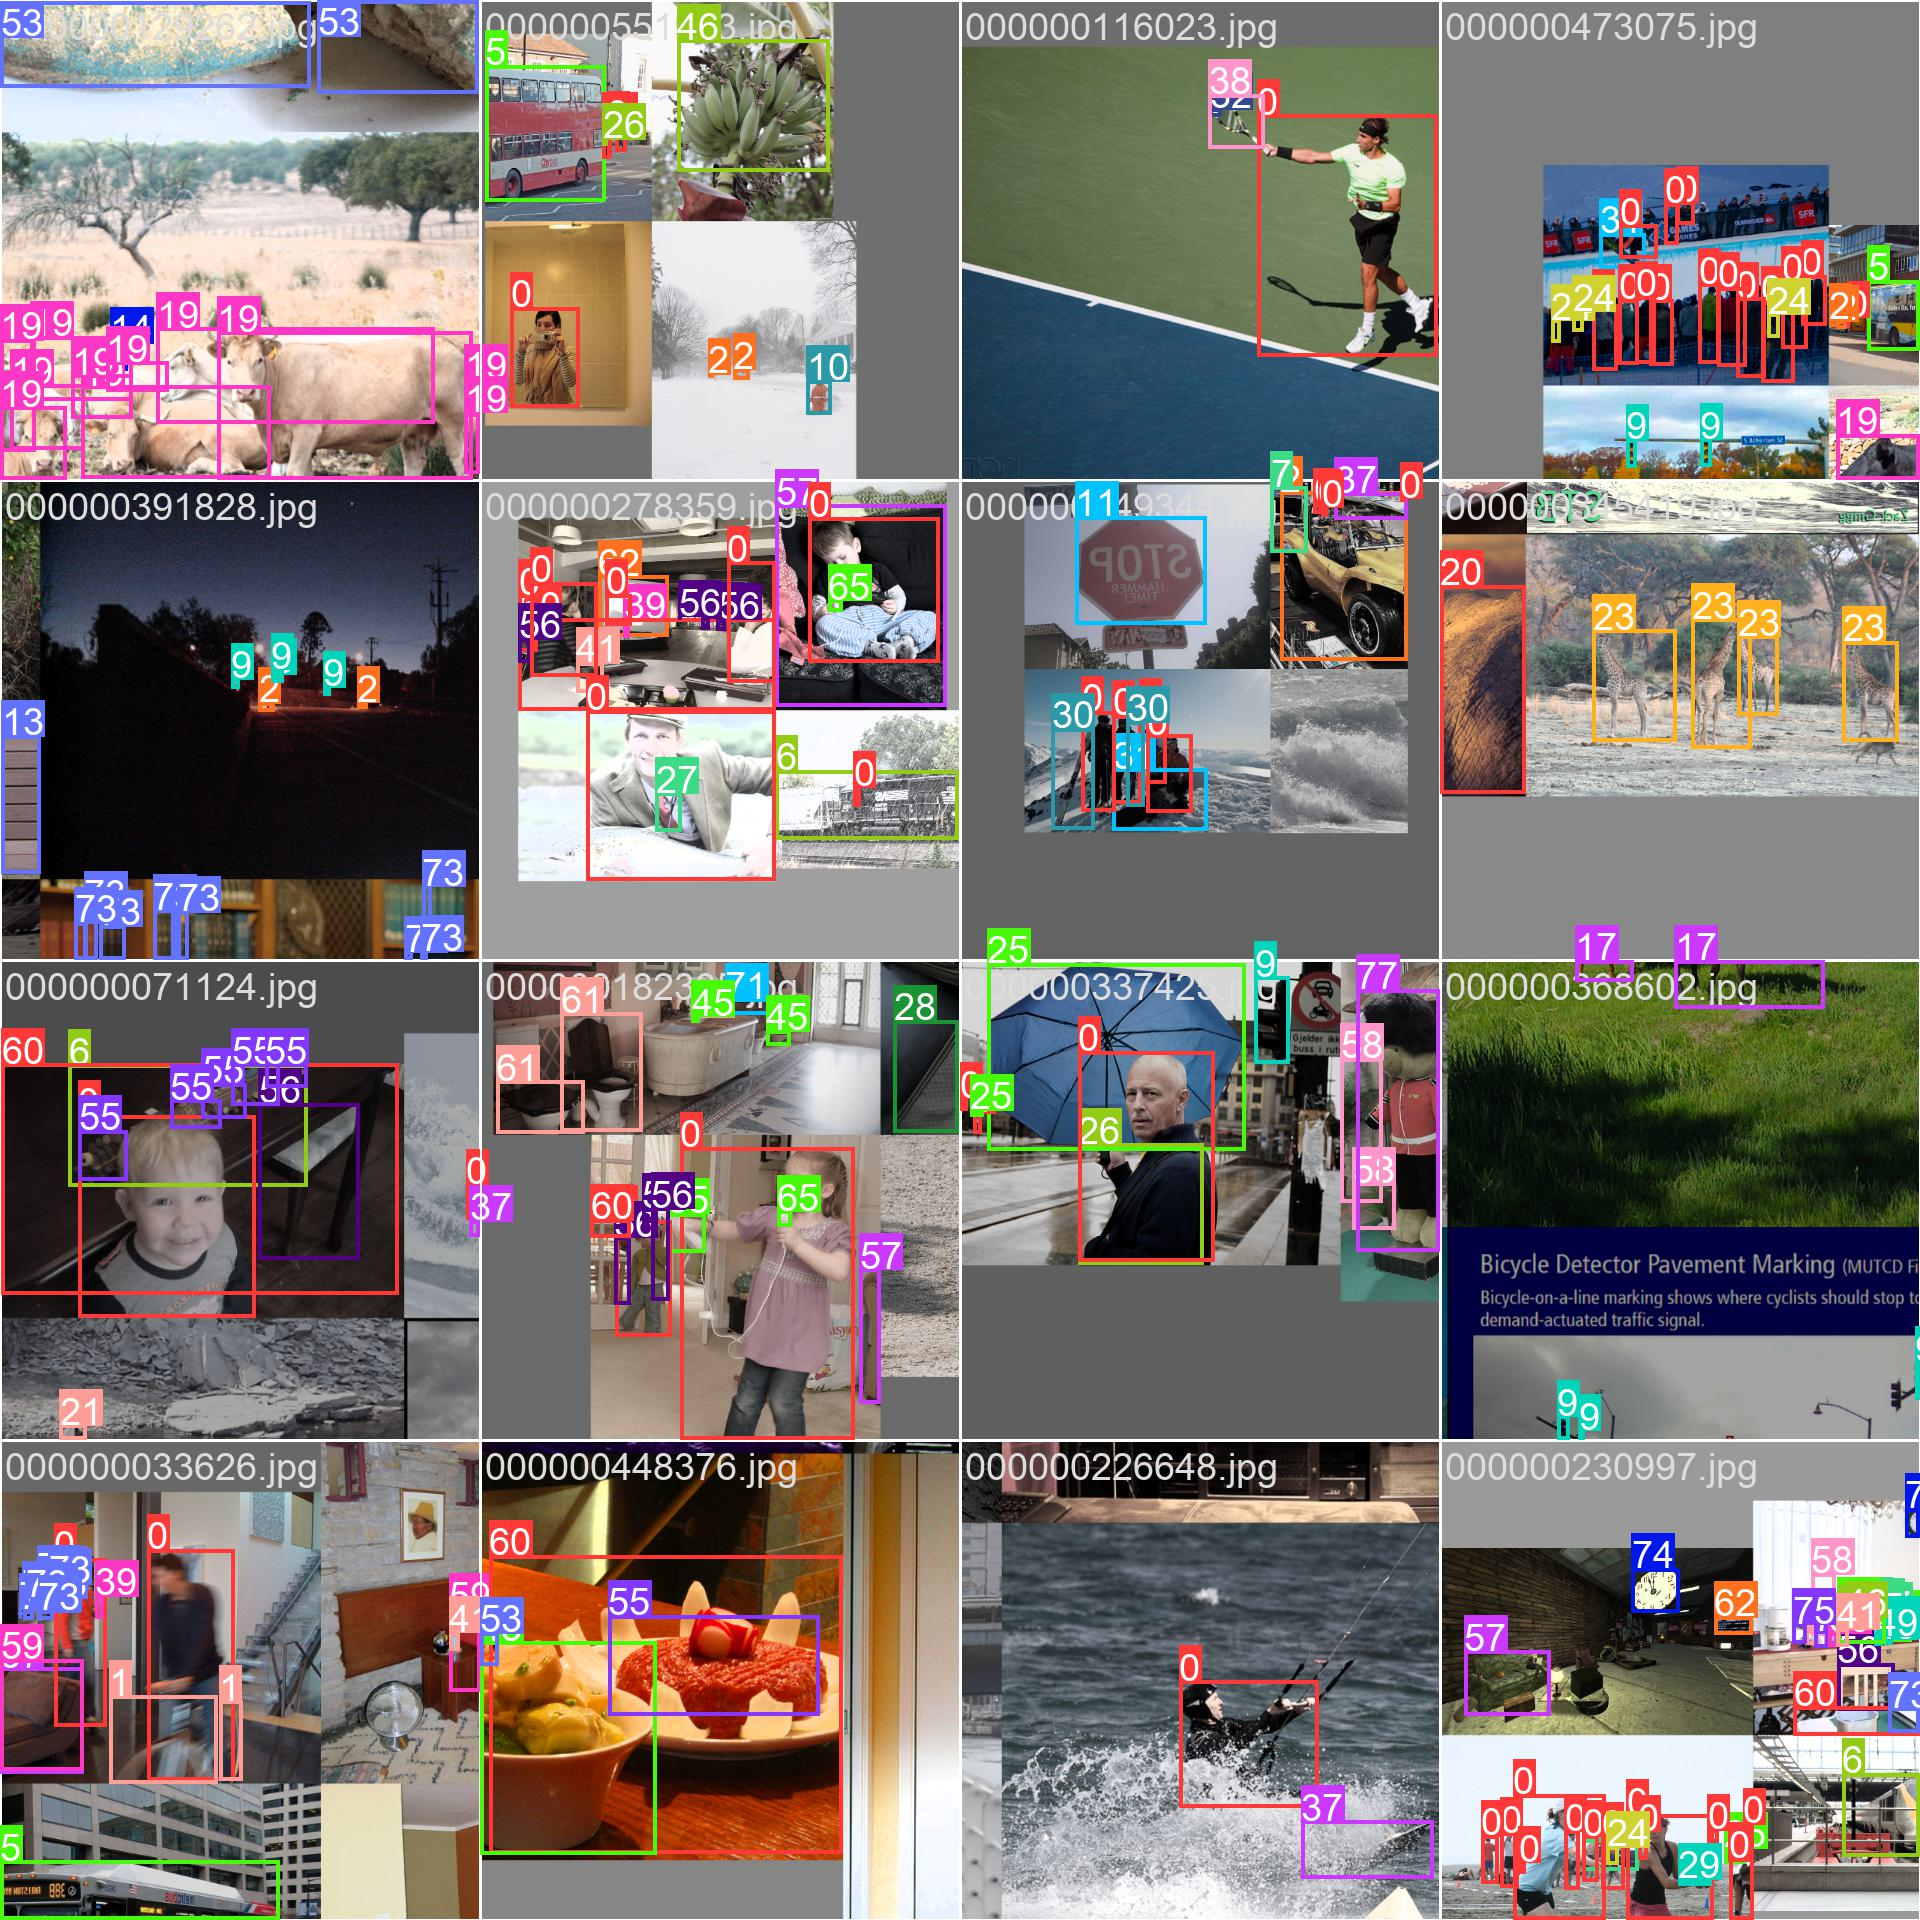
\includegraphics[width=0.8\linewidth]{img/annotations.jpg}
                \caption{Sample Images and Annotations}
                \label{fig:annotations}
            \end{figure}
    \subsection{Training Custom Datasets}
        Download my dataset from my preferred tool. In this example, we use a dataset from Roboflow which is a great annotation platform used by many developers and companies. The dataset is exported in COCO format. \\
        \vspace{3mm}
        In order to train YOLOv9 on my custom dataset, please create a new workflow from scratch. \\
        \vspace{3mm}
        Then I need 2 components:
        \begin{enumerate}
            \item A COCO dataset loader which loads dataset in COCO format and convert it to an Ikomia format
            \item The YOLOv9 training algorithm which loads dataset in Ikomia format
        \end{enumerate}
        \subsubsection{Supported Dataset Formats}
            \begin{figure}[H]
                \centering
                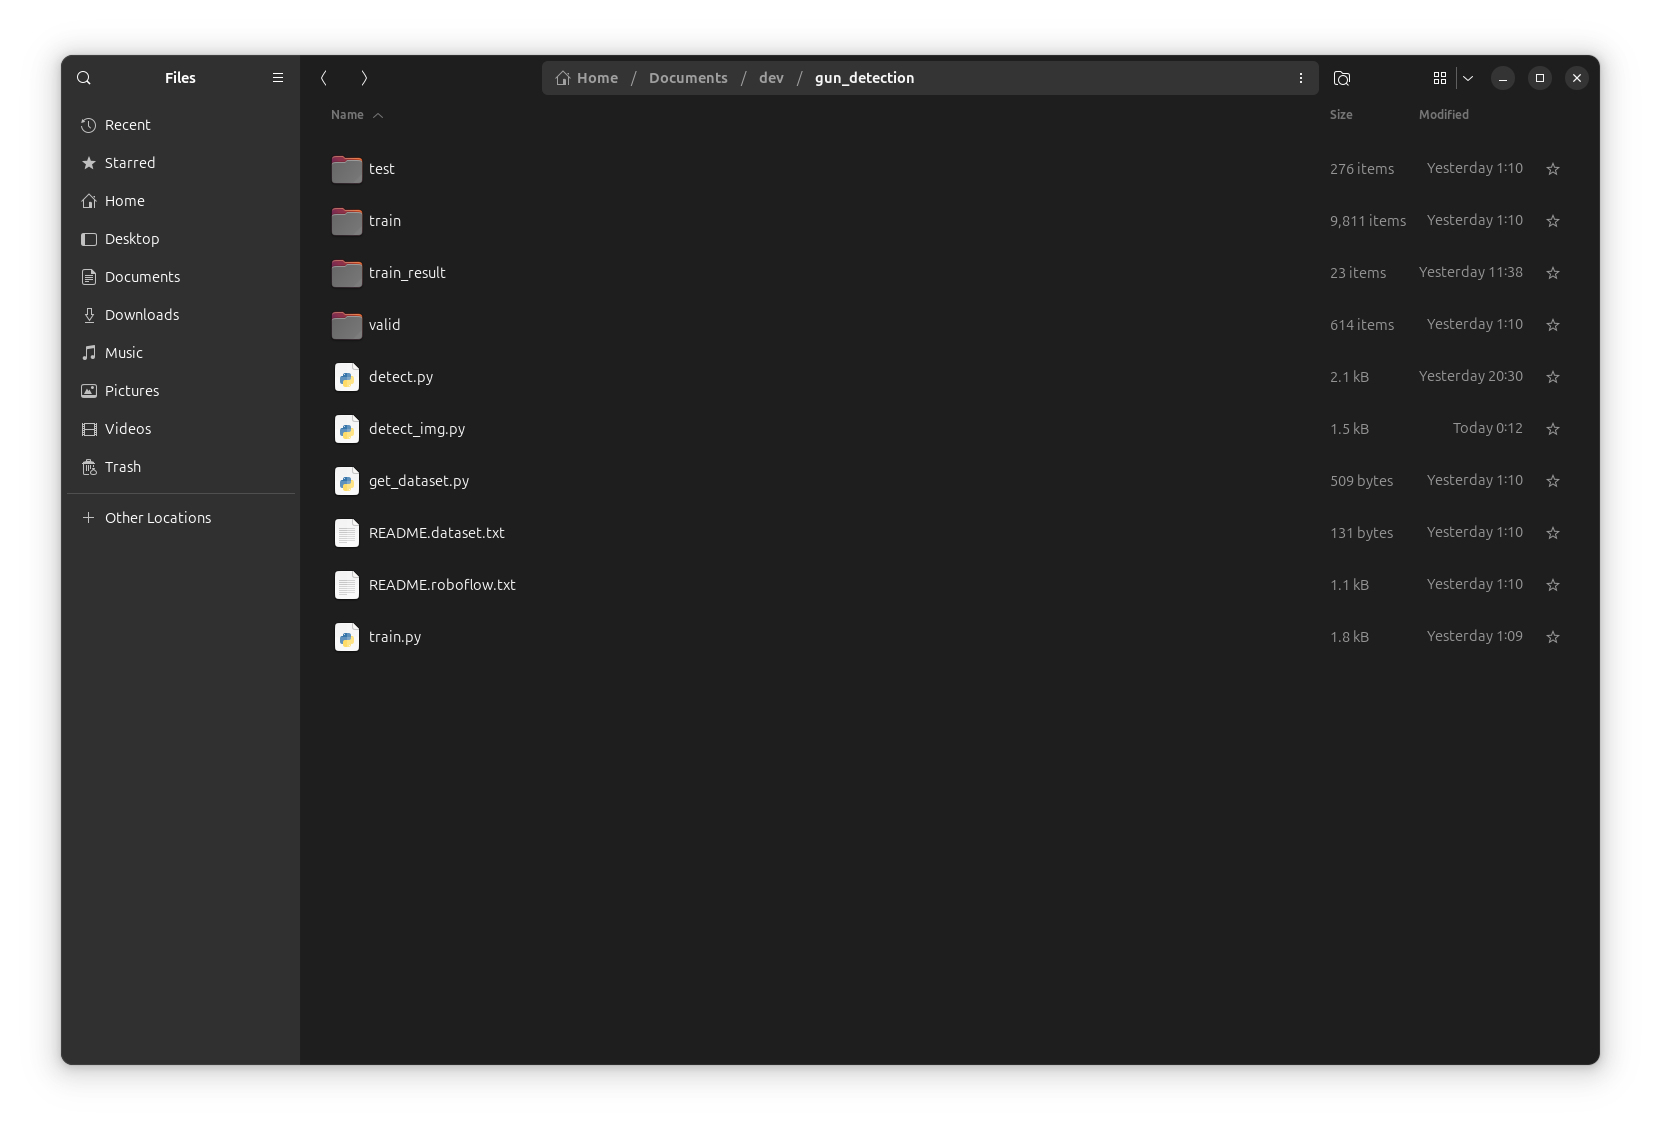
\includegraphics[width=0.8\linewidth]{img/folder_structure.png}
                \caption{COCO Dataset Structure}
                \label{fig:structure}
            \end{figure}
        \subsubsection{Performance on MS COCO Dataset}
            The performance of YOLOv9 on the \textbf{COCO dataset} exemplifies its significant advancements in real-time object detection, setting new benchmarks across various model sizes. Table \ref{tab:object-detector} presents a comprehensive comparison of state-of-the-art real-time object detectors, illustrating YOLOv9's superior efficiency and accuracy.
            \begin{table}[ht]
                \centering
                \small
                \begin{tabular}{| l | l | l | l | l | l |}
                    \hline
                    \rowcolor{lightgray} Model & Size (pixels) & mAP${^{val}_{50:95}}$ & mAP${^{val}_{50}}$ & params (M) & FLOPs (B) \\ \hline
                    YOLOv9t & 640 & 38.3 & 53.1 & 2.0 & 7.7 \\ \hline
                    YOLOv9s & 640 & 46.8 & 63.4 & 7.2 & 26.7 \\ \hline
                    YOLOv9m & 640 & 51.4 & 68.1 & 20.1 & 76.8 \\ \hline
                    YOLOv9c & 640 & 53.0 & 70.2 & 25.5 & 102.8 \\ \hline
                    YOLOv9e & 640 & 55.6 & 72.8 & 58.1 & 192.5 \\ \hline
                \end{tabular}
                \caption{Comparison of State-of-the-Art Real-Time Object Detectors}
                \label{tab:object-detector}
            \end{table}
            YOLOv9's iterations, ranging from the tiny \textbf{\textit{t}} variant to the extensive \textbf{\textit{e}} model, demonstrate improvements not only in accuracy (mAP metrics) but also in efficiency with a reduced number of parameters and computational needs (FLOPs). This table underscores YOLOv9's ability to deliver high precision while maintaining or reducing the computational overhead compared to prior versions and competing models. \\
            \vspace{3mm}
            Comparatively, YOLOv9 exhibits remarkable gains:
            \begin{itemize}
                \item \textbf{Lightweight Models:} YOLOv9s surpasses the YOLO MS-S in parameter efficiency and computational load while achieving an improvement of 0.4$\sim$0.6\% in AP.
                \item \textbf{Medium to Large Models:} YOLOv9m and YOLOv9e show notable advancements in balancing the trade-off between model complexity and detection performance, offering significant reductions in parameters and computations against the backdrop of improved accuracy.
            \end{itemize}
            The YOLOv9c model, in particular, highlights the effectiveness of the architecture's optimizations. It operates with 42\% fewer parameters and 21\% less computational demand than YOLOv7 AF, yet it achieves comparable accuracy, demonstrating YOLOv9's significant efficiency improvements. Furthermore, the YOLOv9e model sets a new standard for large models, with 15\% fewer parameters and 25\% less computational need than YOLOv8x, alongside a incremental 1.7\% improvement in AP. \\
            \vspace{3mm}
            These results showcase YOLOv9's strategic advancements in model design, emphasizing its enhanced efficiency without compromising on the precision essential for real-time object detection tasks. The model not only pushes the boundaries of performance metrics but also emphasizes the importance of computational efficiency, making it a pivotal development in the field of computer vision.
        \subsubsection{Start Training}
            In this work, we will have 4 steps to start training on our custom datasets:
            \begin{enumerate}
                \item \textbf{Step 1:} Create a workflow which will take your dataset as input and train a YOLOv9 model on it
                \item \textbf{Step 2:} First you need to convert the COCO format to IKOMIA format. Add an Ikomia dataset converter to your workflow.
                \item \textbf{Step 3:} Then, you want to train a YOLOv9 model. Add YOLOv9 training algorithm to your workflow
                \item \textbf{Step 4:} Execute your workflow. It automatically runs all your tasks sequentially.
            \end{enumerate}
            \begin{figure}[H]
                \centering
                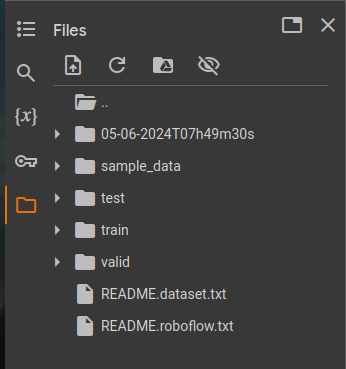
\includegraphics[width=0.8\linewidth]{img/project_tree.png}
                \caption{Project Tree on Colab environment}
                \label{fig:tree}
            \end{figure}
            Model will be trai
            After training finished, we will have an output like below:
            \begin{figure}[H]
                \centering
                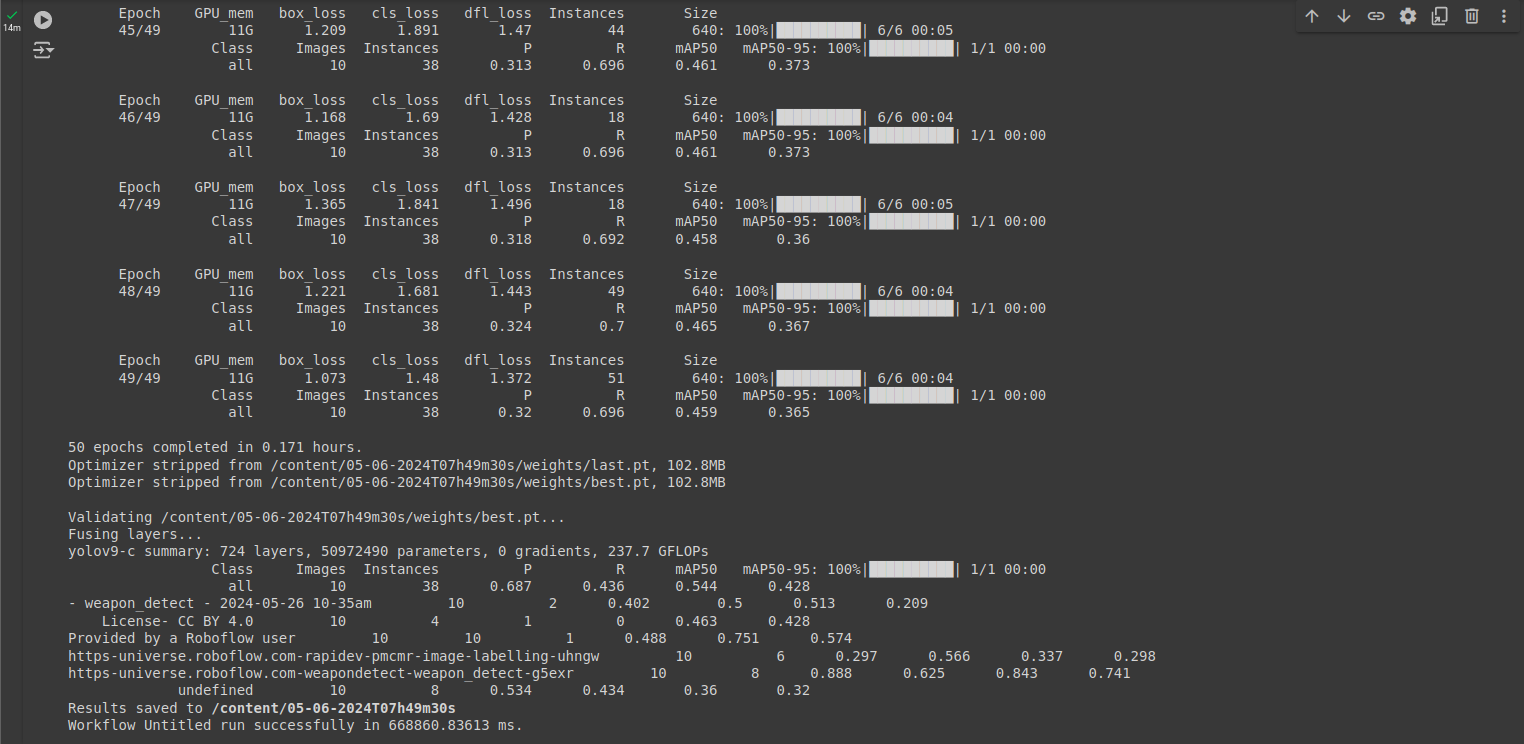
\includegraphics[width=0.8\linewidth]{img/train_result.png}
                \caption{COCO Dataset Training Result}
                \label{fig:train-result}
            \end{figure}
            Model will be trained with 20 epochs. We will do so using the GELAN-C architecture, one of the two architectures released as part of the YOLOv9 GitHub repository. GELAN-C is fast to train. GELAN-C inference times are fast, too. \\
            \vspace{3mm}
            With Google Colab environment, it will be trained with 50 epochs and with 8 batch\_size using 15GB GPU memory, so it just take 15 minutes to complete training process. 
            \begin{figure}[H]
                \centering
                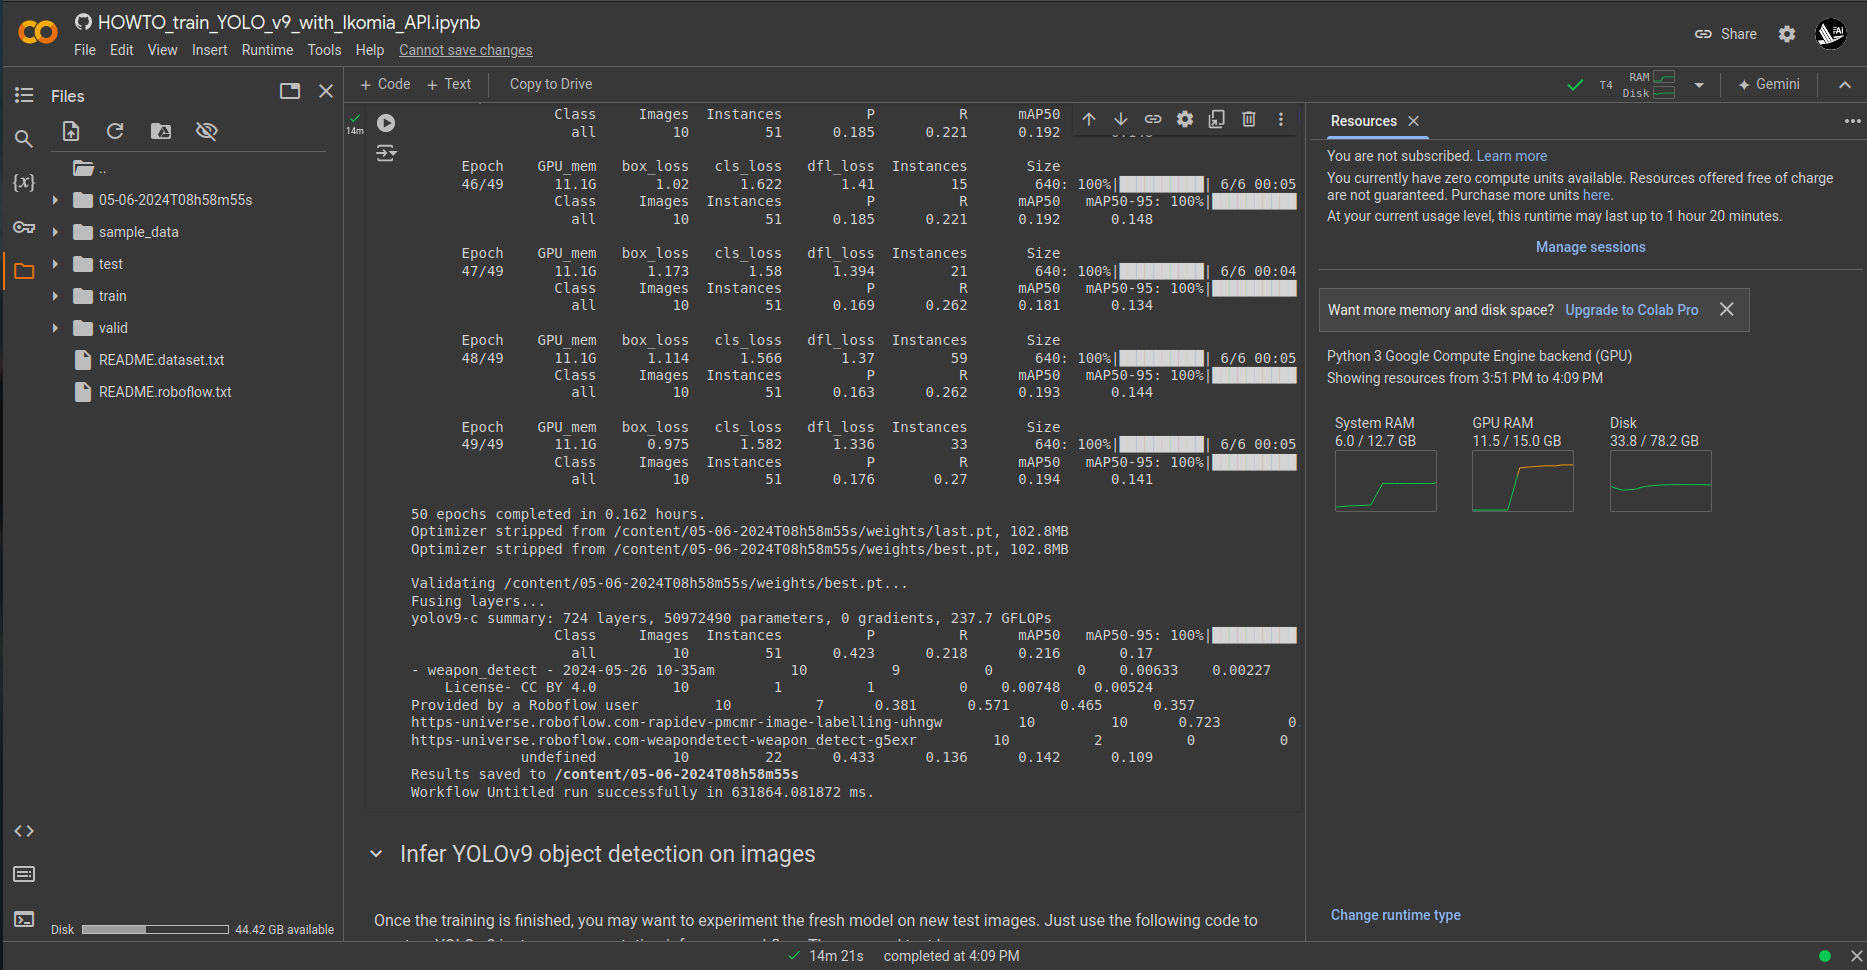
\includegraphics[width=0.8\linewidth]{img/colab_env.png}
                \caption{Google Colab Environment}
                \label{fig:colab-env}
            \end{figure}
            The training process for 20 epochs was completed in approximately 8 hours using an NVIDIA GeForce RTX 3060 12GB GPU. \\
            \vspace{3mm}
            \begin{figure}[H]
                \centering
                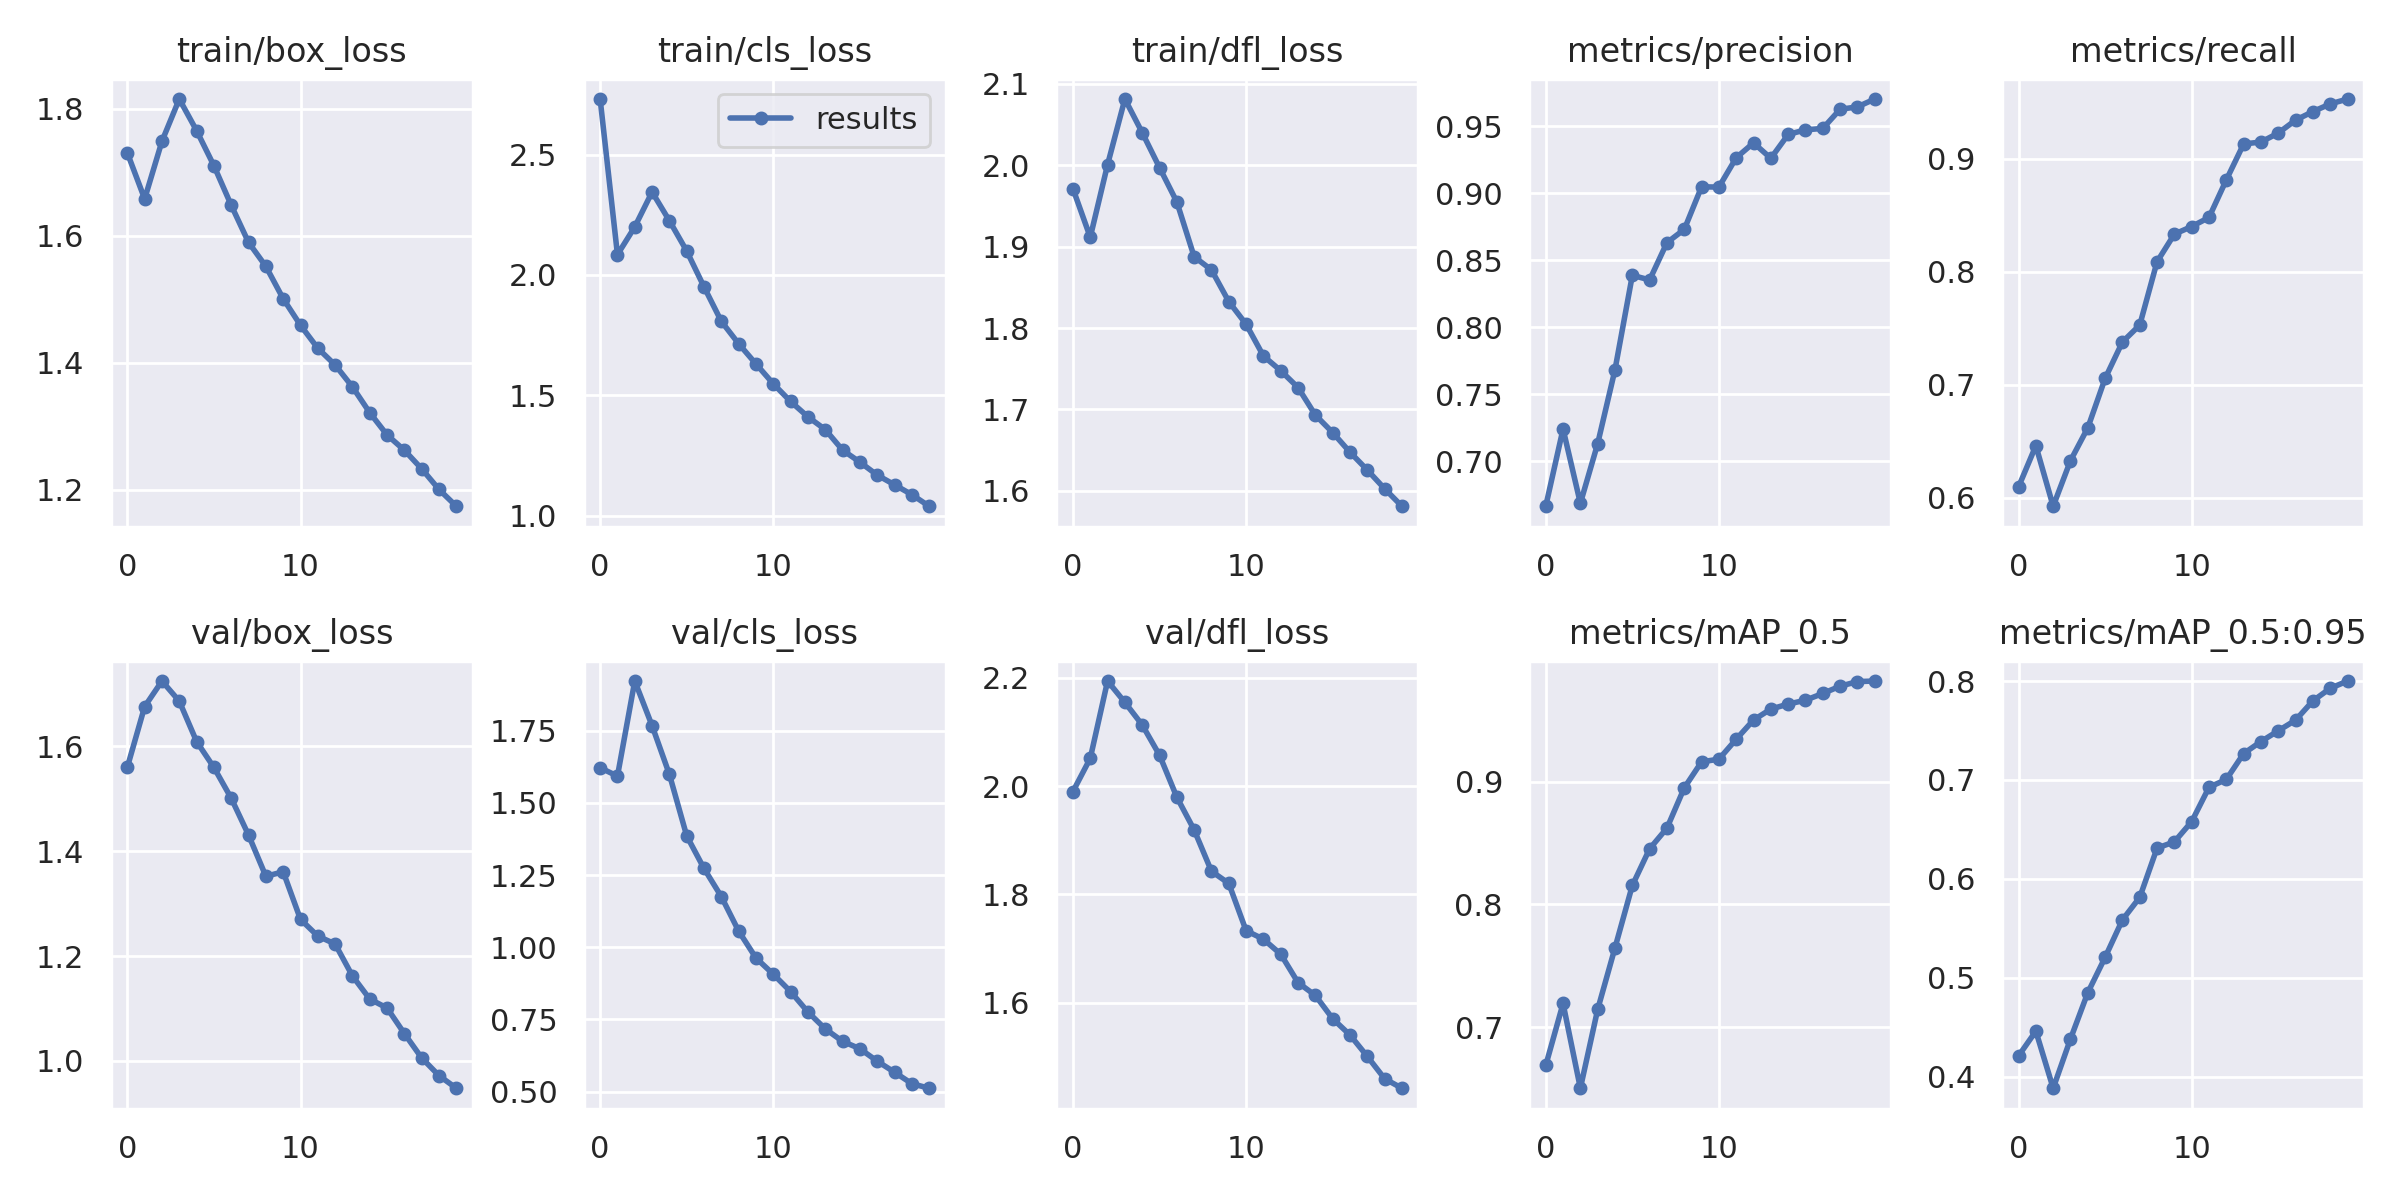
\includegraphics[width=0.8\linewidth]{img/results.png}
                \caption{COCO Dataset Training Graph}
                \label{fig:graph-result}
            \end{figure}
    \subsection{Infer YOLOv9 object detection on images}
        \begin{figure}[H]
            \centering
            \minipage{0.8\textwidth}
                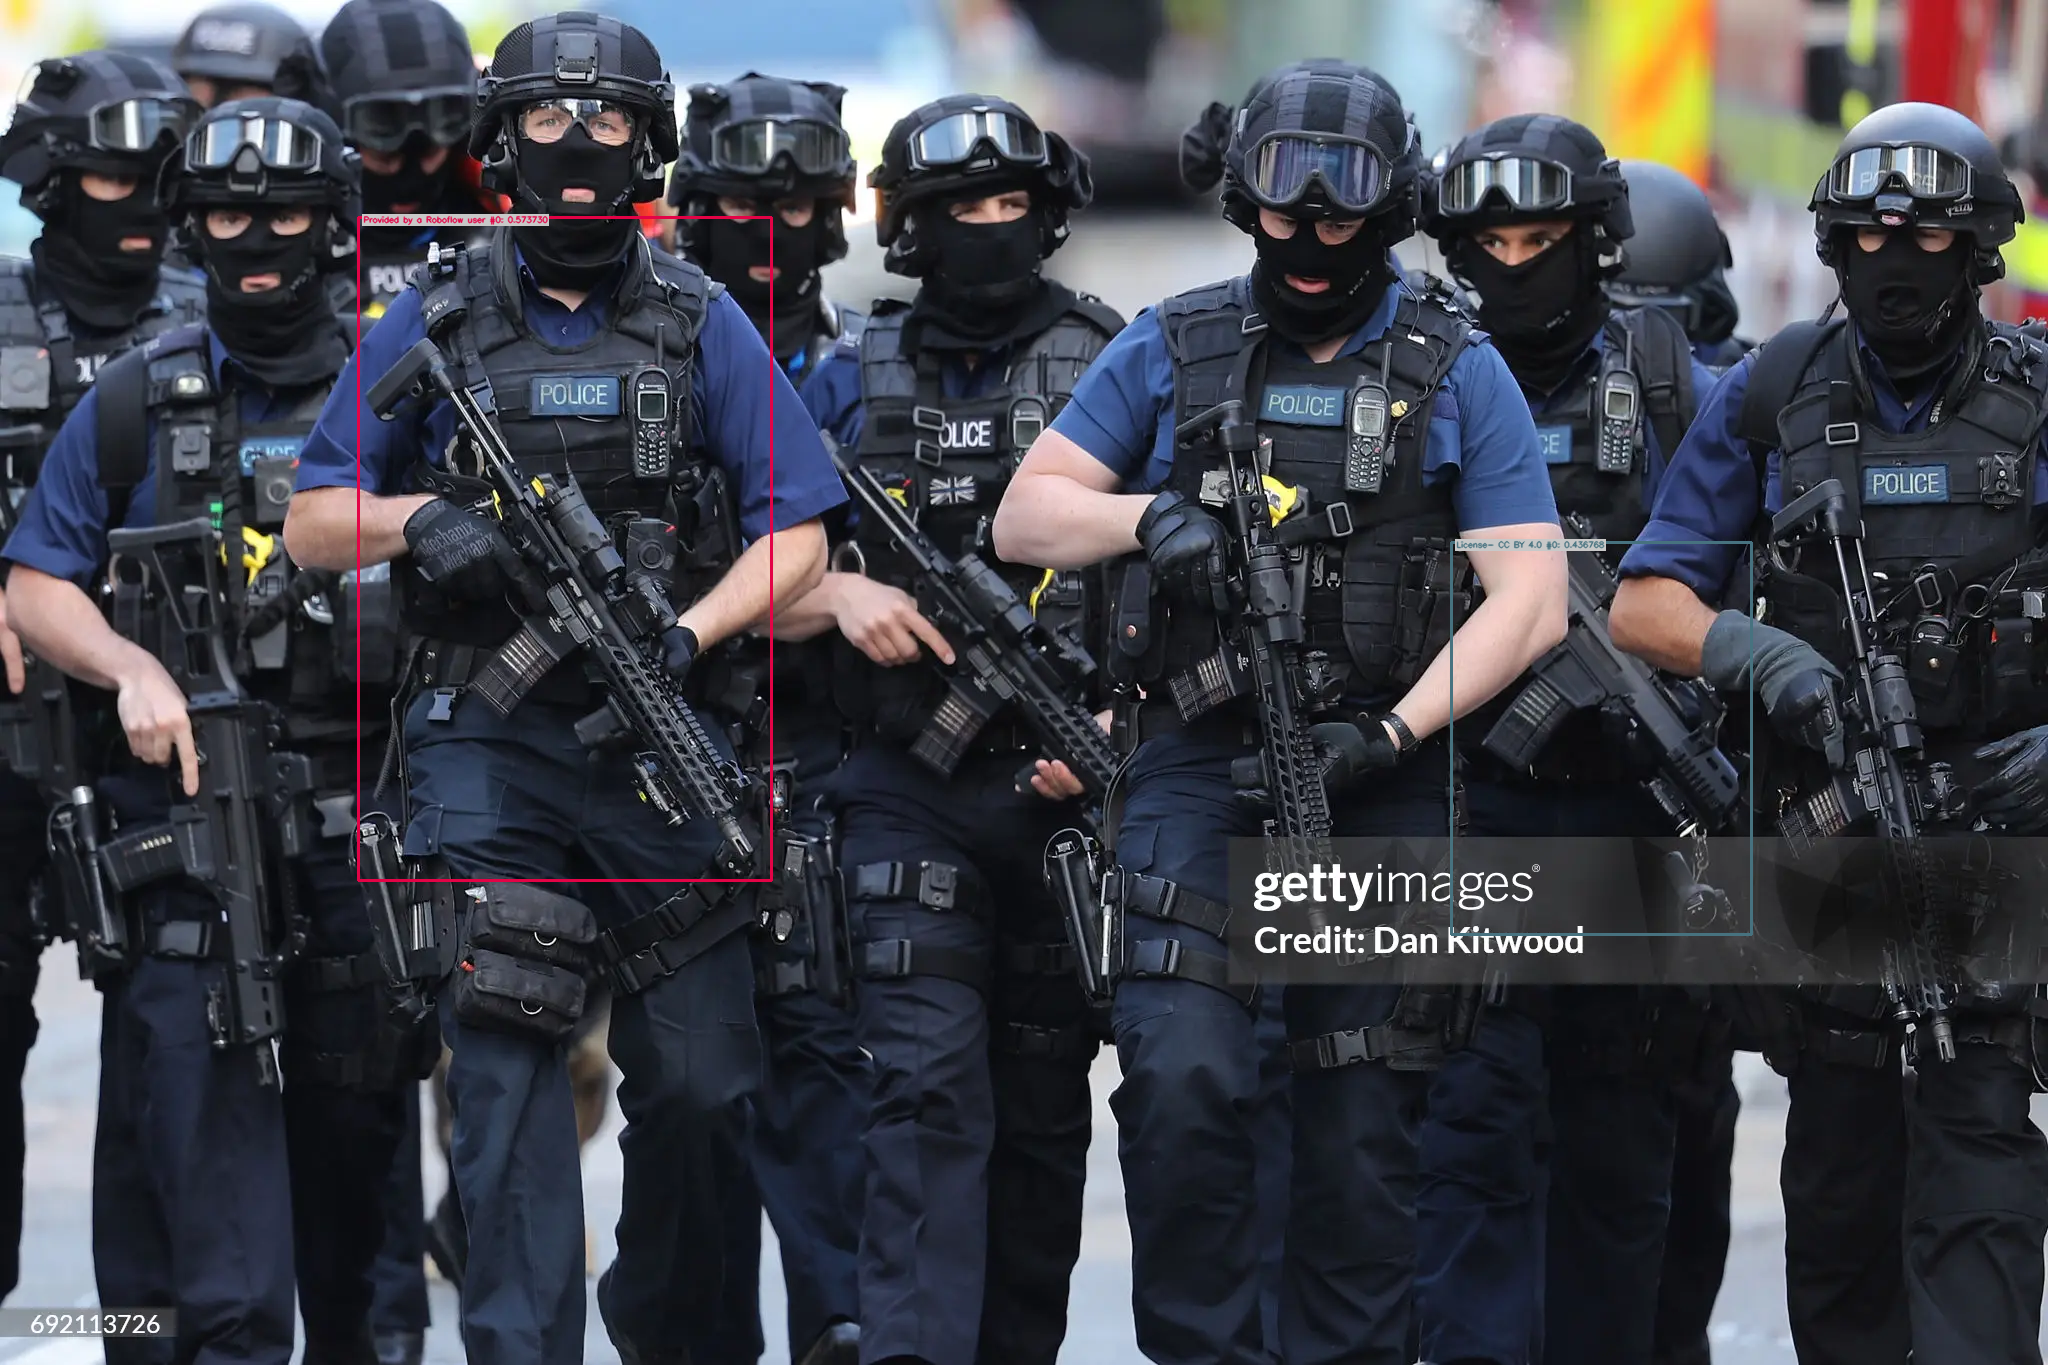
\includegraphics[width=0.8\linewidth]{img/gun_detect.png}
            \endminipage\hfill
            \minipage{0.8\textwidth}%
                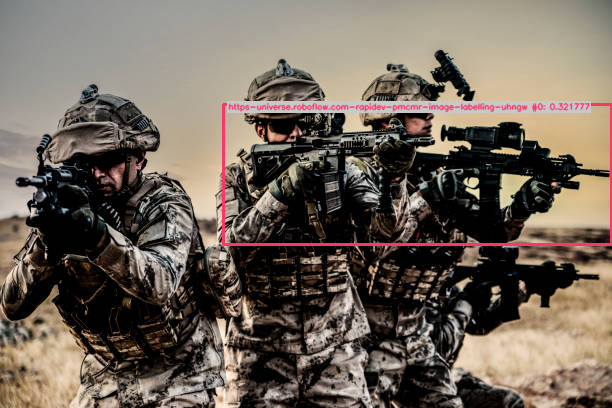
\includegraphics[width=0.8\linewidth]{img/gun_detect_result.png}
            \endminipage\hfill
            \caption{Gun Detect Image Result}
            \label{fig:image-result}
        \end{figure}
    \subsection{Infer YOLOv9 object detection on videos}
        \begin{figure}[H]
            \centering
            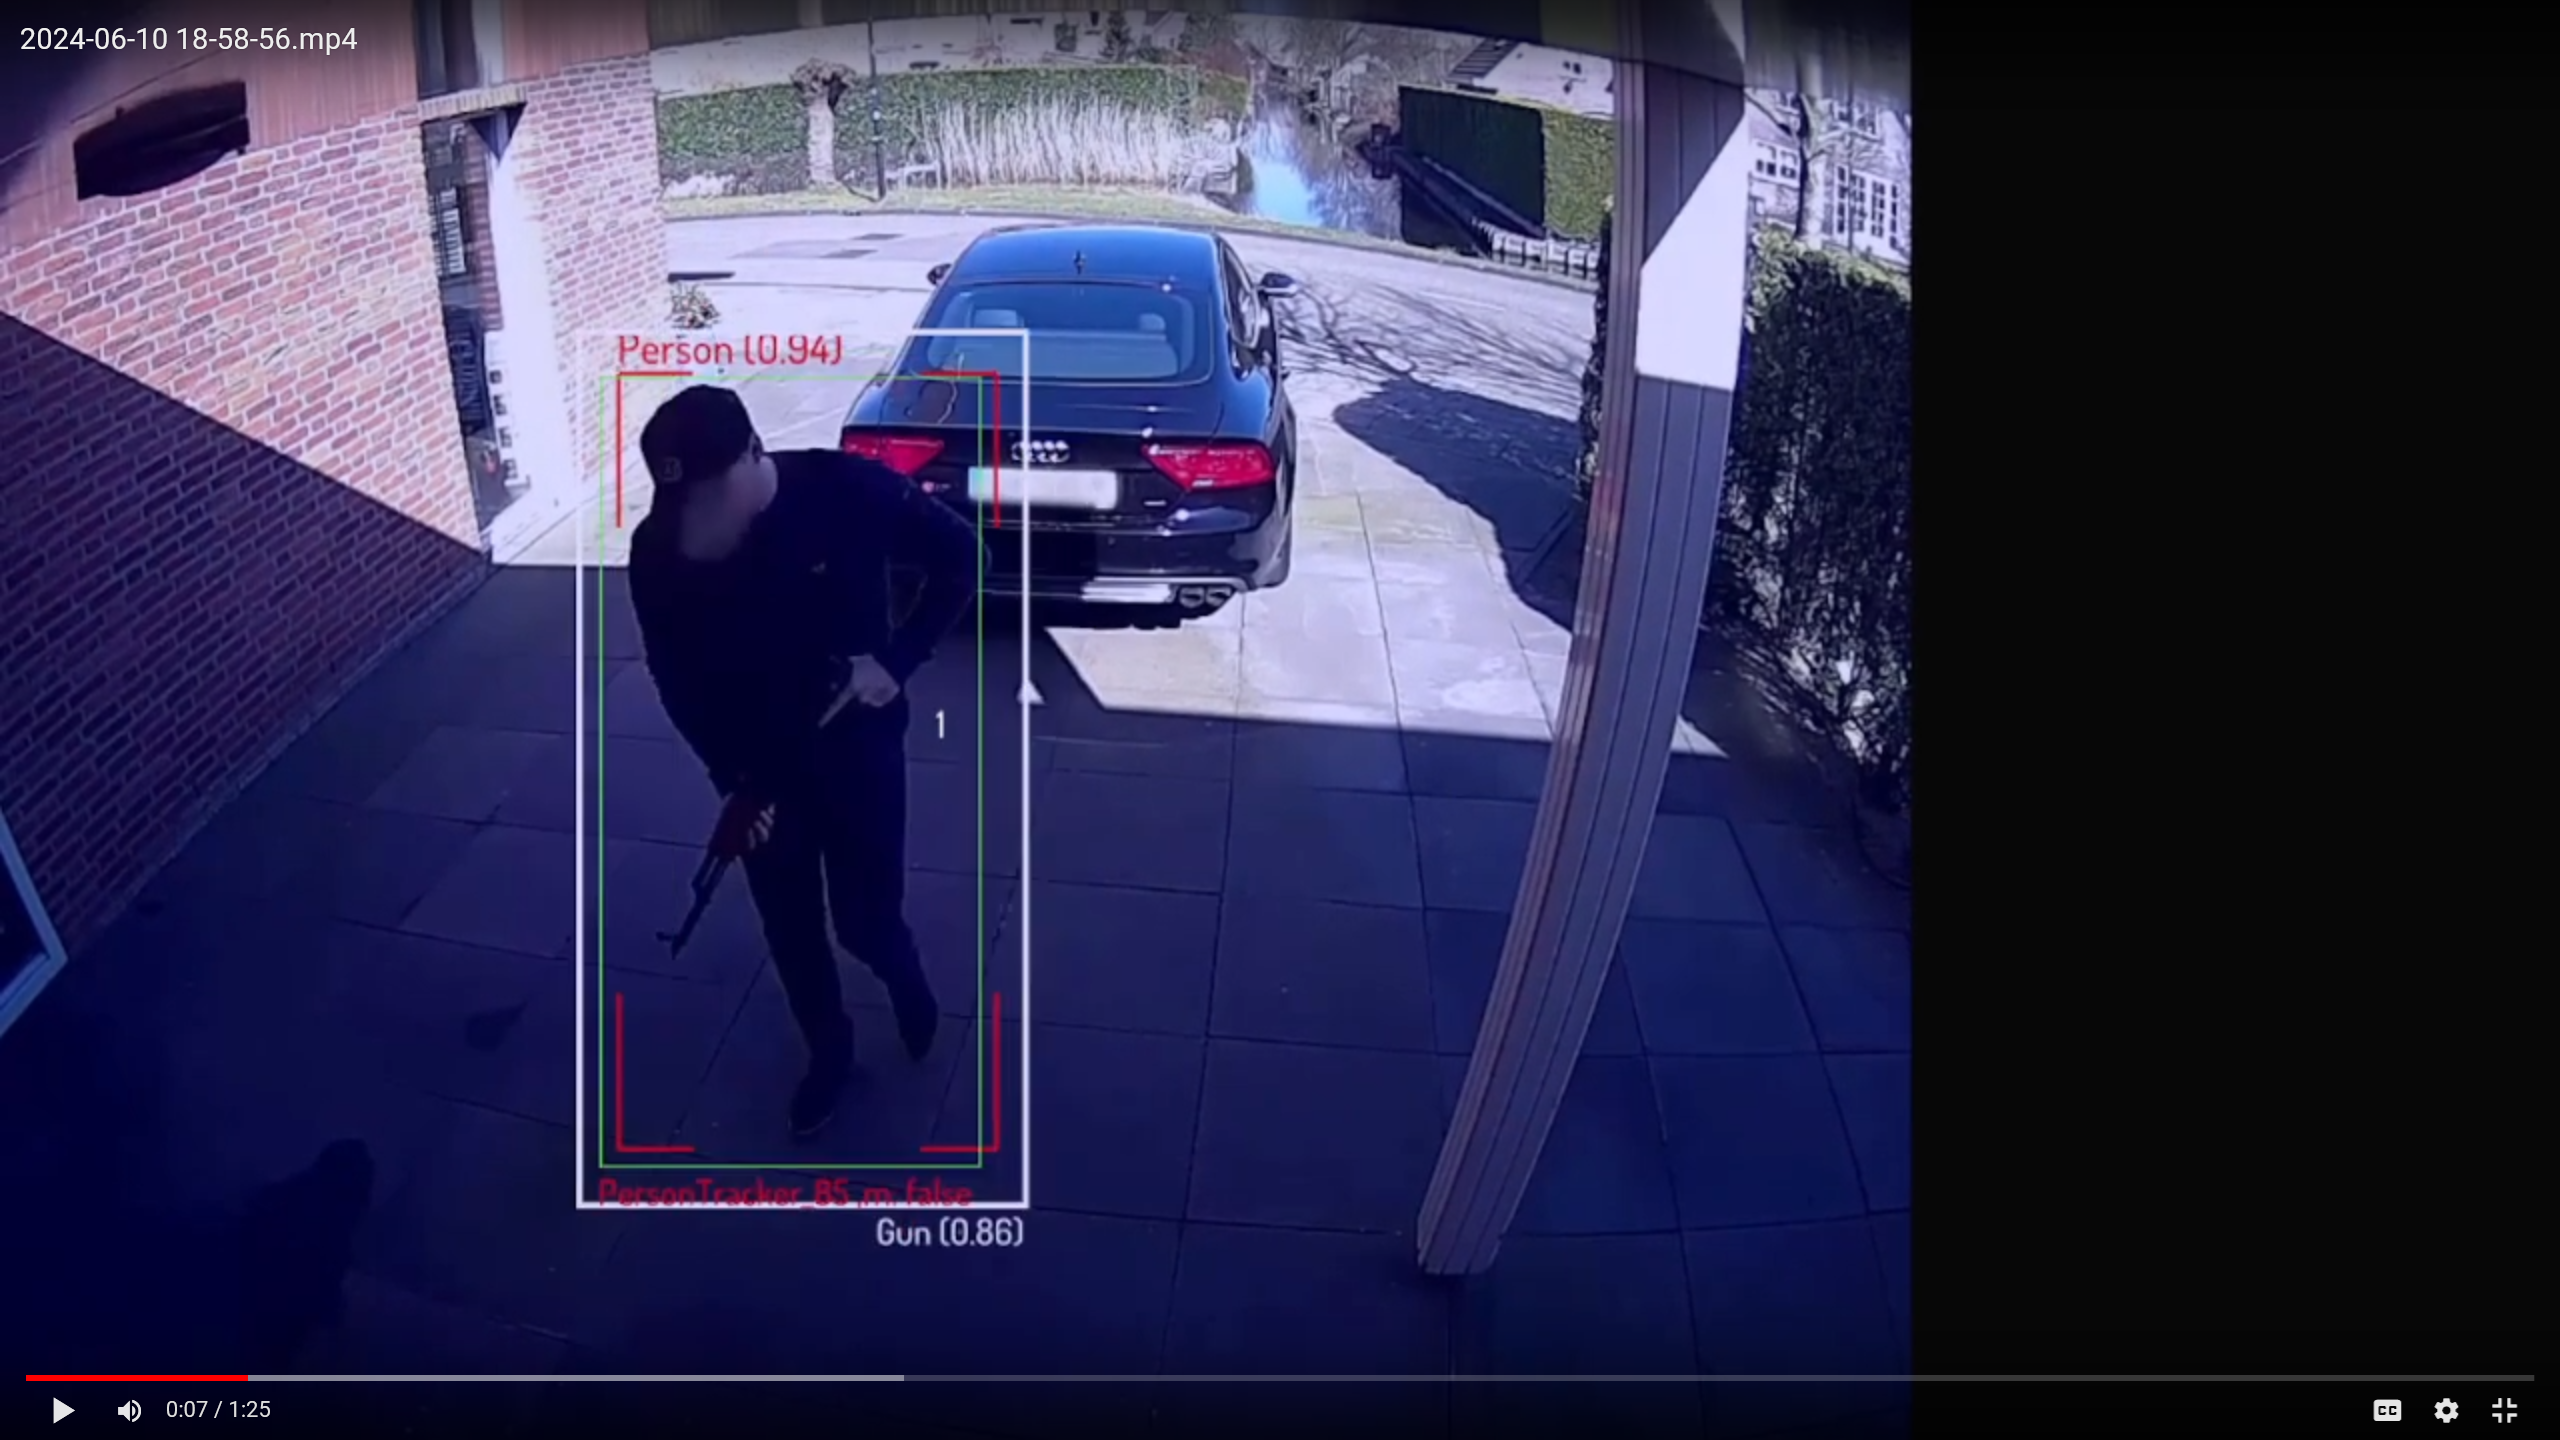
\includegraphics[width=0.8\linewidth]{img/result_data.png}
            \caption{Gun Detect Video Result}
            \label{fig:video-result}
        \end{figure}

    \chapter{CONCLUSIONS}

\renewcommand{\headrulewidth}{0.5pt}
\renewcommand{\footrulewidth}{0.5pt}
\thispagestyle{plain}
\pagestyle{fancy}
\fancyhf{}
\fancyhead[L]{\textbf{CHAPTER 4}}
\fancyhead[R]{\textbf{DANGEGOUS WEAPONS DETECTION USING YOLOv9}}
\raggedright
\fancyfoot[L]{From: Nguyen Van Anh Tuan}
\fancyfoot[R]{Page \thepage}

\justifying

\section{Conclusions}
    In conclusion, the application of YOLOv9 for dangerous weapon detection represents a significant advancement in the field of computer vision and security. YOLOv9's improved accuracy, speed, and robustness make it an ideal solution for real-time weapon detection in various environments such as airports, schools, and public events. The enhanced capabilities of YOLOv9, including better handling of small and overlapping objects, ensure a higher detection rate, thereby increasing the reliability of security systems. By leveraging the latest advancements in deep learning and object detection, YOLOv9 not only enhances the safety of public spaces but also streamlines the process of identifying potential threats, making it an indispensable tool in modern security protocols. As the technology continues to evolve, further integration of YOLOv9 with other security measures will undoubtedly lead to even more effective and comprehensive safety solutions.
\section{Limitations}
    During process of working and implementing with this project, it will be inevitable that there will be some new knowledge and result or experience that i can see from this project. \\
    \vspace{3mm}
    So, in below here, there will be some advantages and disadvantages in this project that i would like to summary. Balancing these advantages and disadvantages is crucial for effective implementation of YOLOv9 in dangerous weapon detection, ensuring that security measures are both efficient and ethical.
    \subsection{Advantages}
        \begin{itemize}
            \item \textbf{High Accuracy:} YOLOv9 offers enhanced accuracy in detecting various types of weapons, reducing false positives and negatives, and ensuring reliable threat identification.
            \item \textbf{Real-time Detection:} The optimized speed of YOLOv9 allows for real-time detection of weapons, which is crucial for timely interventions in security-sensitive environments.
            \item \textbf{Improved Object Handling:} YOLOv9's advanced architecture can better handle small, overlapping, and partially obscured objects, making it more effective in diverse and complex scenarios.
            \item \textbf{Scalability:} YOLOv9 is designed to be scalable and can be deployed on a range of devices from high-end servers to edge devices, making it versatile for various deployment needs.
            \item \textbf{Robustness:} Enhanced generalization capabilities mean YOLOv9 performs well across different datasets and environments, ensuring consistent performance in real-world applications.
            \item \textbf{State-of-the-Art Techniques:} Incorporating the latest advancements in deep learning, YOLOv9 ensures that security systems benefit from cutting-edge technology, providing a future-proof solution.
            \item \textbf{Active Community Support:} Being the latest version, YOLOv9 has robust community support, frequent updates, and comprehensive documentation, facilitating easier implementation and troubleshooting.
        \end{itemize}
    \subsection{Disadvantages}
        \begin{itemize}
            \item \textbf{High Computational Demand:} Despite optimizations, YOLOv9 can still be computationally intensive, requiring powerful hardware for real-time processing, which might not be feasible for all organizations.
            \item \textbf{Complexity in Implementation:} Integrating YOLOv9 into existing security systems may require significant technical expertise and resources, posing a challenge for organizations with limited technical staff.
            \item \textbf{Training Data Requirements:} Achieving high accuracy with YOLOv9 may necessitate large and diverse training datasets, which can be time-consuming and costly to compile and annotate.
            \item \textbf{Potential Privacy Concerns:} Deploying weapon detection systems in public spaces raises privacy concerns, as constant surveillance can be perceived as intrusive, necessitating careful consideration of ethical implications.
            \item \textbf{False Positives and Negatives:} While YOLOv9 improves detection accuracy, no system is flawless. False positives can lead to unnecessary panic and false negatives can pose serious security risks, necessitating human oversight.
            \item \textbf{Maintenance and Updates:} Regular maintenance and updates are required to keep the detection system effective against new types of weapons and evolving threats, which can be resource-intensive.
            \item \textbf{Dependence on Environmental Conditions:} The performance of YOLOv9 can be affected by environmental conditions such as lighting, weather, and camera quality, potentially impacting its effectiveness in certain scenarios.
        \end{itemize}

    \newpage
    \thispagestyle{plain}
    \begin{center}
        \Huge{\textbf{THE REFERENCES}}
    \end{center}
    \vspace{3mm}
    \begin{enumerate}
        \item WongKinYiu, Feb 18th 2024, "\textit{YOLOv9: Learning What You Want to Learn Using Programmable Gradient Information}"
        \item Glenn-Jocher, RizwanMunawar, AyushExel, Created 2023-11-12, Updated 2024-06-10, "\textit{Ultralytics YOLO}"
    \end{enumerate}

    \chapter{APPENDICES}

\renewcommand{\headrulewidth}{0.5pt}
\renewcommand{\footrulewidth}{0.5pt}
\thispagestyle{plain}
\pagestyle{fancy}
\fancyhf{}
\fancyhead[L]{\textbf{CHAPTER 6}}
\fancyhead[R]{\textbf{DANGEGOUS WEAPONS DETECTION USING YOLOv9}}
\raggedright
\fancyfoot[L]{From: Nguyen Van Anh Tuan}
\fancyfoot[R]{Page \thepage}

\justifying

\definecolor{mygray}{rgb}{0.5,0.5,0.5}

\section{Dangerous Weapons Detection Program}

    \lstset{ 
        backgroundcolor=\color{white},   % choose the background color; you must add \usepackage{color} or \usepackage{xcolor}; should come as last argument
        basicstyle=\footnotesize,        % the size of the fonts that are used for the code
        breakatwhitespace=false,         % sets if automatic breaks should only happen at whitespace
        breaklines=true,                 % sets automatic line breakingcommentstyle=\color{mygreen},    % comment style
        captionpos=b,
        deletekeywords={...},            % if you want to delete keywords from the given language
        escapeinside={\%*}{*)},          % if you want to add LaTeX within your code
        extendedchars=true,              % lets you use non-ASCII characters; for 8-bits encodings only, does not work with UTF-8
        firstnumber=1,                % start line enumeration with line 1
        frame=single,	                   % adds a frame around the code
        keepspaces=true,                 % keeps spaces in text, useful for keeping indentation of code (possibly needs columns=flexible)
        keywordstyle=\color{blue},       % keyword style
        language=Python,                 % the language of the code
        morekeywords={*,...},            % if you want to add more keywords to the set
        numbers=left,                    % where to put the line-numbers; possible values are (none, left, right)
        numbersep=5pt,                   % how far the line-numbers are from the code
        numberstyle=\tiny\color{mygray}, % the style that is used for the line-numbers
        rulecolor=\color{black},         % if not set, the frame-color may be changed on line-breaks within not-black text (e.g. comments (green here))
        showspaces=false,                % show spaces everywhere adding particular underscores; it overrides 'showstringspaces'
        showstringspaces=false,          % underline spaces within strings only
        showtabs=false,                  % show tabs within strings adding particular underscores
        stepnumber=1,                    % the step between two line-numbers. If it's 1, each line will be numberedstringstyle=\color{mymauve},     % string literal style
        tabsize=2,	                   % sets default tabsize to 2 spaces
        title=\lstname                   % show the filename of files included with \lstinputlisting; also try caption instead of title
    }

    \begin{lstlisting}[caption={get\_dataset.py}]
        # Import libs
        import requests
        import zipfile
        import os
        
        # Download the file
        #url = "https://universe.roboflow.com/ds/L76hzT4so5?key=tpRs7o81ki"
        url = "https://app.roboflow.com/ds/j1BEJld3NB?key=2PardK2OTb"
        response = requests.get(url, stream=True)
        with open("roboflow.zip", "wb") as file:
            for chunk in response.iter_content(chunk_size=8192):
                file.write(chunk)
        
        # Unzip the file
        with zipfile.ZipFile("roboflow.zip", 'r') as zip_ref:
            zip_ref.extractall()
        
        # Remove the zip file
        os.remove("roboflow.zip")
    \end{lstlisting}

    \begin{lstlisting}[caption={train.py}]
        from ikomia.dataprocess.workflow import Workflow
        import os
        
        try:
            #----------------------------- Step 1 -----------------------------------#
            # Create a workflow which will take your dataset as input and
            # train a YOLOv9 model on it
            #------------------------------------------------------------------------#
            wf = Workflow()
        
            #----------------------------- Step 2 -----------------------------------#
            # First you need to convert the COCO format to IKOMIA format.
            # Add an Ikomia dataset converter to your workflow.
            #------------------------------------------------------------------------#
        
            dataset = wf.add_task(name = "dataset_coco")
        
            dataset.set_parameters({
                "json_file": os.getcwd()+"/train/_annotations.coco.json",
                "image_folder": os.getcwd()+"/train",
                "task":"detection",
                "output_folder": os.getcwd()+"/dataset"
            })
        
            #----------------------------- Step 3 -----------------------------------#
            # Then, you want to train a YOLOv9 model.
            # Add YOLOv9 training algorithm to your workflow
            #------------------------------------------------------------------------#
        
            train = wf.add_task(name="train_yolo_v9", auto_connect=True)
            train.set_parameters({
                "model_name": "yolov9-c",
                "epochs": "20",
                "batch_size": "6",
                "train_imgsz": "640",
                "test_imgsz": "640",
                "dataset_split_ratio": "0.9",
                "output_folder": os.getcwd(),
            })
        
            #----------------------------- Step 4 -----------------------------------#
            # Execute your workflow.
            # It automatically runs all your tasks sequentially.
            #------------------------------------------------------------------------#
            wf.run()
        except Exception as e:
            print(e)
    \end{lstlisting}

    \begin{lstlisting}[caption={detect.py}]
        from ikomia.dataprocess.workflow import Workflow
        from ikomia.utils.displayIO import display
        import cv2
        import os
        
        #video_path = './videos/*.mp4' # Example: https://www.youtube.com/watch?v=EAR5jTknVOw
        video_path = './videos/video_4.mp4'
        output_path = 'output.mp4'
        # Init your workflow
        wf = Workflow()
        
        # Add object detection algorithm
        detector = wf.add_task(name="infer_yolo_v9", auto_connect=True)
        
        detector.set_parameters({
            "model_weight_file": os.getcwd()+ f'/train_result/weights/best.pt',
            "class_file": os.getcwd()+ f'/train_result/classes.yaml',
            "conf_thres": "0.2",
            "iou_thres":"0.25"
        })
        
        # Open the video file
        stream = cv2.VideoCapture(video_path)
        if not stream.isOpened():
            print("Error: Could not open video.")
            exit()
        
        # Get video properties for the output
        frame_width = int(stream.get(cv2.CAP_PROP_FRAME_WIDTH))
        frame_height = int(stream.get(cv2.CAP_PROP_FRAME_HEIGHT))
        frame_rate = stream.get(cv2.CAP_PROP_FPS)
        
        # Define the codec and create VideoWriter object
        # The 'XVID' codec is widely supported and provides good quality
        fourcc = cv2.VideoWriter_fourcc(*'XVID')
        out = cv2.VideoWriter(output_path, fourcc, frame_rate, (frame_width, frame_height))
        
        while True:
            # Read image from stream
            ret, frame = stream.read()
        
            # Test if the video has ended or there is an error
            if not ret:
                print("Info: End of video or error.")
                break
        
            # Run the workflow on current frame
            wf.run_on(array=frame)
        
            # Get results
            image_out = detector.get_output(0)
            obj_detect_out = detector.get_output(1)
        
            # Convert the result to BGR color space for displaying
            img_out = image_out.get_image_with_mask_and_graphics(obj_detect_out)
            img_res = cv2.cvtColor(img_out, cv2.COLOR_RGB2BGR)
        
            # Save the resulting frame
            out.write(img_out)
        
            # Display
            display(img_res, title="YOLOv9 object detection", viewer="opencv")
        
            # Press 'q' to quit the video processing
            if cv2.waitKey(1) & 0xFF == ord('q'):
                break
        
        # After the loop release everything
        stream.release()
        out.release()
        cv2.destroyAllWindows()
    \end{lstlisting}





\end{document}